%-----
% Define o uso do modelo colorido ou preto e branco (escolha uma e descomente)
% Mais abaixo, defina a figura de acordo com a escolha feita.
%-----
\documentclass[a4paper,12pt,brazil]{dct-class}

\usepackage[colorlinks=true]{hyperref}
\usepackage[round]{natbib}
\usepackage{plain}
\usepackage[acronym,toc]{glossaries}

\makeglossaries

\begin{document}
\thispagestyle{empty}
%----- As informa��es abaixo s�o obrigat�rias  ----------------------
%\titulo{Acessibilidade no dom�nio de eGov}
\titulo{Acessibilidade nas fases de Engenharia de Requisitos e Codifica��o de
Software: Uma ferramenta de apoio}
\autor{Rodrigo Gon�alves de Branco}
\doctipo{Disserta��o de Mestrado em Ci�ncia da Computa��o}{}
% Observe que a macro doctipo acima tem 2 par�metros
% O primeiro refere-se ao nome do documento
% O segundo � sua identifica��o num�rica, quando ela existir.
% Use a sintaxe \doctipo{XXXXX}{} quando n�o for
% necess�ria a identifica��o num�rica--------------------------------
%--------------------------------------------------------------------
%--------------------------------------------------------------------
%----- As informa��es abaixo s�o opcionais  -------------------------
\orientacao{ Prof$^a$. Dr$^a$. D�bora Maria Barroso Paiva}
\docarea{Acessibilidade Digital - Engenharia de Software}
\textofree{}
%-----
% Se voc� usa o latex para compilar, comente as figuras do pdflatex
% Defina a figura do grafo a ser utilizada (escolha uma e descomente)
% Fa�a essa escolha de acordo com a classe escolhida (dct-class_bw ou
% dct-class)
%-----
%\vfill \centerline{\includegraphics[scale=0.8]{logo_dct_bw.mps}}
%\vfill \centerline{\includegraphics[scale=0.8]{logo_dct_color.mps}}
%-----
% Se voc� usa o pdflatex para compilar, comente as figuras do latex
% Defina a figura do grafo a ser utilizada (escolha uma e descomente)
% Fa�a essa escolha de acordo com a classe escolhida (dct-class_bw ou
% dct-class)
%-----
%\vfill \centerline{\includegraphics[scale=0.8]{logo_dct_bw-pdflatex.mps}}
%\vfill \centerline{\includegraphics[scale=0.8]{logo_dct_color-pdflatex.mps}}

\vfill \centerline{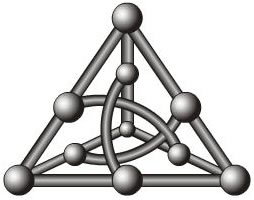
\includegraphics[scale=0.5]{logo_dct.jpg}}

%--------------------------------------------------------------------
% O trecho seguinte n�o pode ser mudado ou retirado -----------------
\vskip 0.5cm
\begin{center}
        Faculdade de Computa��o - FACOM\\
        Universidade Federal de Mato Grosso do Sul\\
        \today
\end{center}
%\newpage

\chapter*{}

\begin{center}

\begin{minipage}[t]{10cm}
  \begin{center}
\vspace{-2cm}
    {{\Large Acessibilidade nas fases de Engenharia de Requisitos e Codifica��o de
Software: Uma ferramenta de apoio}}  
  \end{center}
\end{minipage}
\end{center}

% \begin{flushright}
% \begin{minipage}[t]{6cm}
% \vspace{2cm}
%     {Este exemplar corresponde � reda��o final da disserta��o devidadamente corrigida e defendida por
% Rodrigo Gon�alves de Branco e aprovada pela Banca Examinadora.}  
% \end{minipage}
% \end{flushright}

\begin{flushright}
\vspace{12cm}
Campo Grande, \today.
\end{flushright}

\vspace{2cm}
Banca Examinadora:

\begin{itemize}
  \item Prof$^a$. Dr$^a$. D�bora Maria Barroso Paiva (FACOM/UFMS) - orientadora
  \item ????
  \item ????
\end{itemize}

%----------------------------------------------------------------------

\chapter*{Agradecimentos}

Aos meus pais, que, apesar de nunca terem entendido complemtamente o que fa�o em
minha �rea profissional, sempre me apoiaram e continuam me apoiando. Agrade�o
por me mostrarem desde cedo o valor dos estudos, e por serem exemplos a qual
pretendo continuar seguindo.

� minha esposa Juliana, que, no come�o deste trabalho era apenas namorada, mas
n�o menos importante por este motivo. Agrade�o pela motiva��o excepcional que
sempre me forneceu, por me tolerar e compartilhar os momentos de adversidade que surgiram
nesta caminhada, bem como tamb�m os momentos felizes. E, principalmente, pelo
apoio em todas as decis�es que tomei at� agora.

Ao meu irm�o, Leandro, por ser o companheiro e camarada que ele sempre foi,
sempre disposto a me acompanhar, seja l� qual fosse o programa. Agrade�o tamb�m
por ser esta pessoa de extrema paci�ncia, sempre calmo, independente da situa��o
envolvida.

� minha professora e orientadora, professora D�bora, por sempre acreditar em meu
trabalho. Agrade�o pela paci�ncia, orienta��es e conselhos oferecidos durante
essa longa trajet�ria, me ajudando desde os tempos de minha
gradua��o, n�o me abandonando nem mesmo quando precisei me mudar para uma cidade
muito distante como Porto Velho, me incentivando sempre a continuar em minha
jornada no programa de Mestrado.

Ao meu sobrinho Enzo, apenas por existir, e alegrar minha vida com seus
sorrisos, sua voz e suas brincadeiras.

Aos meus amigos e colegas de faculdade, que sempre ajudaram a deixar minha vida
mais divertida, fazendo-me esquecer, mesmo que por pouco tempo, dos problemas cotidianos.
Agrade�o tamb�m aos meus amigos que tamb�m compartilharam de momentos ruins da
minha vida e ainda assim estavam l� para me apoiar e consolar.

A todos os meus professores da FACOM e do programa de Mestrado, profissionais
que tenho orgulho em dizer que foram meus tutores, cujos ensinamentos carrego comigo at� hoje e tento
compartilhar com os demais.

Aos meus colegas de trabalho, passando pelo TJ-MS, IFMS e atualmente no TRT-RO,
por me mostrar a imensid�o de opini�es, t�cnicas e abordagens encontradas em
nossa �rea de atua��o. Agrade�o a estes por me mostrar o que realmente � cobrado
e quais as melhores forma de encarar u 

A todos que compartilharam direta ou indiretamente para o desenvolvimento deste
trabalho.


\chapter*{Resumo}

Fornecer produtos acess�veis deixou a pouco tempo de ser um diferencial de
determinadas empresas. Acessibilidade, nos dias atuais, � um requisito fundamental de qualquer solu��o desenvolvida, indicando principalmente
respeito e cumplicidade com os clientes. Essa afirma��o � especialmente
verdadeira para os produtos desenvolvidos para a \textit{Internet}, porta de
acesso para toda a intercomunica��o mundial. A \textit{Internet} se mostrou a
tecnologia mais r�pida e barata de aquisi��o de informa��o, levando tecnologias
legadas (servi�os banc�rios, por exemplo) a se adaptarem de forma que pessoas
com dificuldades permanentes ou moment�neas consigam interagir com a sociedade.
Contudo, fornecer um produto acess�vel nem sempre � uma tarefa f�cil. Al�m de
diversas classes diferentes de defici�ncias e dificuldades (o que acarreta
problemas de acessibilidade diferentes), a falta de treinamento e experi�ncia na
�rea faz com que desenvolvedores cometam erros em v�rios aspectos, resultando
num produto inacess�vel. Os modelos de processos e \textit{frameworks} de desenvolvimento de
\textit{software} ainda n�o se adaptaram de forma consistente e homog�nea,
em rela��o a acessibilidade na f�brica de \textit{software}. A �rea de
Tecnologia da Informa��o est� passando por uma fase de transi��o entre o
\textit{HTML 4 e XHTML} para o \textit{HTML 5}, que, entre outras coisas, pretende entregar uma \textit{web} sem�ntica e
tratar dos problemas espec�ficos de acessibilidade, mas que ainda n�o est�
plenamente consolidada. Por fim, as ferramentas dispon�veis aos desenvolvedores
n�o conseguem, de maneira eficaz, auxiliar efetivamente os desenvolvedores a
entregarem um produto acess�vel. Neste trabalho, pretende-se resolver o
problema do escasso suporte ao desenvolvimento de \textit{softwares} acess�veis
presente nas ferramentas de constru��o de \textit{software} dispon�veis,
construindo um \textit{plugin} para o \textit{Eclipse}, uma \textit{IDE
(Integrated Development Environment)} altamente customiz�vel e extens�vel
utilizada por muitos desenvolvedores em todo o mundo.

\label{resumo}
\chapter*{Abstract}

Providing accessible products has recently left  to be a differential
feature of certain companies. Accessibility, today, is a fundamental requirement
of any developed solution, indicating primarily respect and care to
customers.
This statement is especially true for products designed to the Internet which is
the gateway of all  world intercommunication. The Internet has showed to be the
fastest and cheapest technology to acquire information, and has forced legacy
technologies (banking services, for example) to adapt itself so that people with
permanent or momentary difficulties can be able to interact with society.
However, to give an accessible product is not always an easy task. In addition to several different classes of disabilities / difficulties (which leads to
different accessibility problems), lack of training and experience in the area
makes developers producing code in a wrong way, resulting in an inaccessible
product.
The process models and software development frameworks have not been adapted in a
consistent and homogeneous way, contemplating the accessibility in the software
factory. We are going through a transition phase between from the HTML and
XHTML 4 to HTML 5, which among other things, aims to deliver a semantic web and
to treat specific problems of accessibility, but it's not yet fully
consolidated.
Finally, the tools available to developers cannot effectively assist developers to
deliver an affordable product. In this work it is considered that the accessibility requirements should be taken into account during all phases of software development, ie, must evolve from initial requirements analysis to the phase of software testing in order to obtain accessibility as an attribute of software quality of the final product. Thus, we sought primarily to create an approach that could promote accessibility requirements traceability from conception to the coding phase. This approach has associated Requirements, UML models and implementation techniques for accessibility, mapped in an accessibility ontology. In addition, we developed a plugin for Eclipse that promoted the association of technical implementation of accessibility and traceability matrix.

\textbf{Keywords:} \textit{accessibility, requirement traceability,
software development process, CASE tool.}

\label{abstract}

%--------------------------------------------------------------------
% Aqui come�a a inclus�o dos seus textos
%
\renewcommand{\contentsname}{Sum�rio} % renomeando o contentsname
\renewcommand*{\glossaryname}{Gloss�rio}
\deftranslation{Glossary}{Gloss�rio}
\tableofcontents{}
%---- O comando abaixo deve ser usado caso queira incluir o conte�do
%como bookmark, visando facilitar a navega��o no Acrobat Reader
%---------------------------------------------------------------------
\addcontentsline{toc}{chapter}{Sum�rio}\label{sumario}
%---------------------------------------------------------------------
%------ Aqui devem ser inclu�dos os cap�tulos ------------------------

\newacronym{rup}{RUP}{Rational Unified Process}
\newacronym{xp}{XP}{eXtremming Programming}
\newglossaryentry{scrum}{name=SCRUM,description={Nome baseado em um jogada do
jogo de Rubgy, onde o jogo � reiniciado ap�s uma pequena infra��o}}
\newglossaryentry{wysiwyg}{name=WYSIWYG,description={What You See Is What You
Get, usados para softwares que mostram as altera��es feitas em documentos em
tempo real, de maneira fiel ao resultado final}}
\newacronym{php}{PHP}{Hypertext Preprocessor}
\newacronym{www}{WWW}{World Wide Web}
\newacronym{dda}{DDA}{Disability Discrimination Act}
\newacronym{ietf}{IETF}{The Internet Engineering Task Force}
\newacronym{w3c}{W3C}{World Wide Web Consortium}
\newacronym{wai}{WAI}{Web Accessibility Initiative}
\newacronym{wcag}{WCAG}{Web Content Accessibility Guidelines}
\newacronym{wai-aria}{WAI-ARIA}{Accessible Rich Internet Applications Suite}
\newacronym{atag}{ATAG}{Authoring Tool Accessibility Guidelines}
\newacronym{uaag}{UAAG}{User Agent Accessibility Guidelines}
\newacronym{earl}{EARL}{Evaluation and Report Language}
\newglossaryentry{w3c-wai}{name=W3C-WAI,description={Ramifica��o da W3C que
trata de aspectos relacionados a acessibilidade na Internet}}
\newacronym{clf}{CLF}{Common Look and Feel}
\newacronym{nda}{NDA}{National Disability Authority}
\newacronym{emag}{e-MAG}{Modelo de Acessibilidade de Governo Eletr�nico}
\newacronym{idh}{IDH}{�ndice de Desenvolvimento Humano}
\newglossaryentry{cms}{name=CMS,description={Content Management Systems,
ferramenta de autoria utilizada para publica��o de portais}}
\newacronym{ajax}{AJAX}{Asynchronous JavaScript and XML}
\newacronym{dhtml}{DHTML}{Dynamic HTML}
\newacronym{html}{HTML}{HyperText Markup Language}
\newacronym{http}{HTTP}{HyperText Transfer Protocol}
\newacronym{xml}{XML}{Extensible Markup Language}
\newacronym{smil}{SMIL}{Synchronized Multimedia Integration Language}
\newacronym{rdf}{RDF}{Resource Description Framework}
\newacronym{lip}{LIP}{Learner Information Package}
\newacronym{acclip}{ACCLIP}{Accessibility for LIP}
\newacronym{accmd}{ACCMD}{AccessForAll Meta-data}
\newacronym{ims}{IMS}{IMS Global Learning Consortium}
\newacronym{dp}{DP}{Device Profile}
\newacronym{nfr}{NFR}{Non-Functional Requeriments}
\newacronym{ar}{AR}{Accessibility Requeriments}
\newacronym{https}{HTTPS}{HyperText Transfer Protocol Secure}
\newacronym{xhtml}{XHTML}{eXtensible Hypertext Markup Language}
\newacronym{javacc}{JavaCC}{Java Compiler Compiler}
\newacronym{rss}{RSS}{Really Simple Syndication}
\newacronym{xslt}{XSLT}{eXtensible Stylesheet Language for Transformation}
\newacronym{xpath}{XPath}{XML Path Language}
\newacronym{css}{CSS}{Cascade Style Sheet}
\newacronym{j2me}{J2ME}{Java Plataform Micro Edition}
\newacronym{ugc}{UGC}{User-generated Content}
\newacronym{uwem}{UWEM}{Unified Web Evaluation Methodology}
\newacronym{waqm}{WAQM}{Web Accessibility Quantitative Metric}
\newacronym{wab}{WAB}{Web Accessibility Barriers}
\newacronym{pm}{PM}{Page Measurement}
\newacronym{up}{UP}{Unified Software Development Process}
\newacronym{case}{CASE}{Computer-Aided Software Engineering}
\newacronym{uml}{UML}{Unified Modeling Language}
\newacronym{owl}{OWL}{Web Ontology Language}
\newacronym{birt}{BIRT}{Business Intelligence Reporting Tools}
\newacronym{ibm}{IBM}{International Business Machines}
\newacronym{emf}{EMF}{Eclipse Modeling Framework}
\newacronym{ide}{IDE}{Integrated Development Environment}
\newacronym{mta}{MTA}{Modelo de Taferas de Acessibilidade}
\newacronym{rmf}{RMF}{Requirements Modeling Framework}

%\addcontentsline{toc}{chapter}{Gloss�rio}\label{glossario}

\printglossary

\listoffigures

\listoftables

\chapter{Introdu��o}

\pagenumbering{arabic}

\setcounter{page}{1}

\section{Contexto e Motiva��o}

A utiliza��o de sistemas para internet � cada vez mais comum. Atividades que
antes eram realizadas presencialmente est�o migrando para servi�os virtuais que
podem ser acessados a partir de qualquer dispositivo com acesso � internet.

A Receita Federal Brasileira, por exemplo, s� recebe as declara��es de Imposto
de Renda via internet \citep{irpf:13}. As declara��es emitidas em
papel foram completamente abandonadas no ano de 2011
\citep{irpf:11}. Essa decis�o foi tomada pois a declara��o feita em papel � mais
vagarosa em todos os aspectos se comparada ao envio da declara��o pela Internet e, al�m disso, era muito grande o n�mero de declara��es preenchidas 
erroneamente usando os formul�rios impressos \citep{irpf_estacao:11}.

Alguns Tribunais j� instituiram a emiss�o de certid�es apenas por meio
eletr�nico. Um exemplo � o Tribunal de Justi�a do Estado do Cear�, que permite a
emiss�o de Certid�o Negativa Criminal por meio de seu \textit{site}
\citep{tjce:11}. Segundo o pr�prio Tribunal, os motivos para adotar a emiss�o de
Certid�o \textit{online} implicam em ``rapidez, transpar�ncia, amplo acesso, interatividade e significativa redu��o
de custos materiais e humanos, contribuindo para os resultados de excel�ncia que
se pretende alcan�ar na presta��o dos servi�os do Judici�rio � popula��o''
\citep{tjce_portaria:11}.

O Conselho Monet�rio Nacional autorizou uma medida que permite que os bancos
possam oferecer aos seus clientes uma conta movimentada exclusivamente por meios
eletr�nicos. Assim, o cliente ficar� isento de cobran�as de tarifas caso fa�a
movimenta��es usando canais eletr�nicos, como Internet, caixas
eletr�nicos e celular \citep{jc:11}.

Os exemplos citados mostram a import�ncia da Internet na dissemina��o de
informa��o e fornecimento de diversos servi�os. A Internet h� muito tempo n�o �
tratada mais como uma ferramenta de luxo ou acess�ria, mas sim como uma
ferramenta essencial nas atividades do cotidiano das pessoas. H� v�rias
vantagens em se usar a Internet para apoiar a comunica��o e os neg�cios das
empresas, por exemplo \citep{oliveira:11}:

\begin{itemize}
  \item Disponibilidade de 24 horas por dia;
  \item Possibilidade de acesso de todas as partes do planeta;
  \item Necessidade de espa�o f�sico e de infra-estrutura reduzidos (ex: bancos)
  para realizar as atividades;
  \item Custo de investimento inicial baixo, etc.
\end{itemize}

Todos deveriam ter pleno acesso aos recursos
fornecidos pela Internet. No entanto, devido a dificuldades e defici�ncias de
determinados grupos de pessoas, o acesso aos recursos pode ficar comprometido,
sendo que em algumas situa��es sequer o acesso � poss�vel. � necess�rio,
portanto, fornecer maneiras de garantir a acessibilidade de informa��es e servi�os da
\textit{Internet}.

\cite{5260918} definem Acessibilidade Digital como o requisito b�sico para
fornecer um acesso equalit�rio � informa��o extra�da da \textit{Internet},
principalmente e especialmente por ser uma maneira vital de acesso ao conte�do
por grupos vulner�veis (principalmente pessoas com necessidades especiais).
Necessidades especiais n�o se referem apenas a pessoas com defici�ncia f�sica
ou mental, mas tamb�m a pessoas com algum tipo de impossibilidade moment�nea,
como a navega��o atrav�s de um \textit{browser} textual ou a visualiza��o de um
\textit{site} atrav�s de um \textit{smartphone}, que possui suas dimens�es reduzidas.

Entregar produtos acess�veis n�o � uma tarefa f�cil. O assunto �
considerado relativamente recente e est� sendo alvo de muitas pesquisas
\citep{lazar:04,brajnik:06,zeng:05}. A acessibilidade na \textit{web} tamb�m j�
� regulamentada em v�rios pa�ses, com diretivas e boas pr�ticas que norteiam sua
aplica��o. Por isso, o papel da Engenharia de \textit{Software} neste contexto �
fundamental. A falta de metodologia e processos bem definidos espec�ficos para acessibilidade podem
gerar produtos n�o acess�veis. Os custos s�o menores quando a
acessibilidade � considerada durante o processo de desenvolvimento do
\textit{software} \citep{groves:11}. Apesar de existir um custo impl�cito
embutido (por exemplo, contrata��o de um especialista em acessibilidade,
ferramentas pr�prias para testes em acessibilidade, etc), em geral, os
benef�cios alcan�ados pela incorpora��o da acessibilidade nos processos s�o
maiores do que os custos envolvidos necess�rios para a entrega do produto,
pois o custo de manuten��o posterior geralmente � mais alto e h� um acr�scimo no
valor agregado ao produto \citep{sherman:01}.

Existem propostas para integrar usabilidade
e acessibilidade aos processos de Engenharia de \textit{Software}
\citep{springerlink:10.1007/978-3-642-02713-0,maia:10}. Outras propostas s�o
espec�ficas para determinadas plataformas \citep{microsoft:09}. Contudo, n�o s�o
encontrados na literatura trabalhos que integram acessibilidade a modelos e
\textit{frameworks} de desenvolvimento bem conhecidos, como \gls{up}
\citep{Jacobson:1999:USD:309683}
(ou sua extens�o mais conhecida
\gls{rup} \citep{rup:13}), \gls{xp}
\citep{Beck:1999:EPE:318762} ou Scrum \citep{DeGrace:1990:WPR:83202}.

T�o importante quanto integrar acessibilidade no processo de desenvolvimento de
\textit{software} s�o as compet�ncias t�cnicas do Engenheiro de
Software, Analista de Sistemas, Projetista e Desenvolvedor.
Devido a fatores como a recente exposi��o do tema nos meios de comunica��o e a defici�ncia no treinamento e forma��o do desenvolvedores,
muitos deles sequer sabem como codificar para tornar seus produtos acess�veis
\citep{1630123, alves:11}. As v�rias classes de problemas de acessibilidade
contribuem para tornar o trabalho de codifica��o ainda mais dif�cil. A utiliza��o de
componentes de \textit{software} com atributos de qualidade embutidos (sistemas
de gerenciamento de conte�do e sistemas \textit{wiki} normalmente possuem um
editor \gls{wysiwyg} que j� s�o acess�veis, como o
\textit{TinyMCE} \citep{tinymce:13}) atenuam mas n�o eliminam o problema. A
conscientiza��o dos desenvolvedores v�m ocorrendo de forma gradual, mas poucas institui��es de ensino brasileiras dedicam uma disciplina espec�fica para Acessibilidade, ou dedicam pouco tempo em disciplinas de �mbito maior como Interface
Humano-Computador, Hiperm�dia/Multim�dia ou Engenharia de \textit{Software}
(Exemplos de grades curriculares:
Harvard\footnote{http://www.seas.harvard.edu/teaching-learning/undergraduate/computer-science/planning-and-courses},
MIT\footnote{http://ocw.mit.edu/courses/electrical-engineering-and-computer-science/\#undergrad},
USP\footnote{http://www.ime.usp.br/dcc/grad/grade},
UFMS\footnote{http://www.sien.ufms.br/cursos/grade/1904} e
IFMS\footnote{http://www.ifms.edu.br/rightsidebar/cursos/graduacao-2/tecnologia-em-sistemas-para-internet/}).

A utiliza��o de ferramentas que ap�iam os profissionais na constru��o de boas
solu��es acess�veis � muito comum, pois aumenta a produtividade, retirando boa
parte do esfor�o necess�rio e diminuindo passos repetitivos que seriam
necess�rios sem o aux�lio de tais ferramentas. Em geral, s�o utilizadas
ferramentas \textit{CASE, IDEs e frameworks}, mas existem algumas ferramentas
espec�ficas para o contexto de acessibilidade. Existem v�rias classes destas
ferramentas espec�ficas, entre elas:

\begin{itemize}
  \item simulador: a ferramenta simula uma defici�ncia/dificuldade, mostrando ao
  desenvolvedor o problema do produto \citep{5358165};
  \item validador: a ferramenta utiliza um conjunto de normas e padr�es
  pr�-definidos e, atrav�s da valida��o objetiva, julga se o produto atende ou
  n�o aos crit�rios definidos\footnote{Exemplo de validador da W3C:
  http://validator.w3.org/};
  \item avaliador: a ferramenta utiliza um validador, complementando com
  informa��es, dicas e m�tricas, al�m de apresentar potenciais problemas que
  devem ser verificados manualmente\footnote{Exemplo de avaliadores:
  Hera(http://www.sidar.org/hera/) e daSilva(http://www.dasilva.org.br/)}.
\end{itemize}

Os avaliadores s�o ferramentas �teis, utilizados para fiscaliza��o e
auditoria de \textit{sites}. Por�m, pesquisas mostram que os desenvolvedores n�o
est�o satisfeitos com os avaliadores dispon�veis
\citep{Trewin:2010:ACT:1805986.1806029}. As ferramentas nem sempre informam de
forma objetiva as mudan�as necess�rias para fornecer um produto acess�vel
\citep{groves:12}. Desenvolvedores iniciantes podem n�o entender as informa��es
apresentadas na ferramenta. E, principalmente, os desenvolvedores est�o
insatisfeitos em utilizar ferramentas externas ao seu ambiente de desenvolvimento
para efetuar a avalia��o \citep{Trewin:2010:ACT:1805986.1806029}.

A situa��o � agravada pela constata��o de que h� poucos estudos que abordam a
engenharia de requisitos e rastreabilidade do ponto de vista do t�pico
acessibilidade, ou seja, poucos estudos t�m indicado como ocorre a evolu��o dos requisitos
de acessibilidade durante o processo de desenvolvimento das aplica��es web \citep{analuizadias:2010}.

\section{Objetivos}

Diante do exposto, os objetivos deste trabalho s�o:

\begin{enumerate}
  \item Estender o \gls{mta} (tratado na se��o \ref{chapter:mta}),
  propondo uma metodologia para a rastreabilidade dos requisitos de acessibilidade
  atrav�s do processo de desenvolvimento de \textit{software};
  \item Permitir a associa��o expl�cita entre os requisitos de
  acessibilidade e os artefatos de documenta��o e, para cada associa��o,
  especificar uma ou mais t�cnicas de implementa��o de acessibilidade de acordo com o documento de conformidade em acessibilidade escolhido;
  \item Implementar uma ferramenta de suporte que seja integrada ao ambiente de
  desenvolvimento e que implemente os objetivos listados acima.
\end{enumerate}

Busca-se identificar pontos de integra��o entre as etapas de engenharia de
requisitos, projeto e implementa��o de c�digo e propor uma ferramenta (\textit{plugin} Eclipse) que represente esta
integra��o. Assim, pretende-se que os requisitos de acessibilidade se tornem
itens de acessibilidade verific�veis e o desenvolvedor dever� ser
informado se a associa��o requisitos, modelos e c�digo est� ou n�o sendo feita. A ferramenta dever�
apresentar sugest�es para que os itens de acessibilidade sejam implementados.
Com isso, pretende-se desenvolver uma ferramenta de apoio � acessibilidade
diferente daquelas apresentadas na literatura, pois ter� como foco a acessibilidade durante o processo de desenvolvimento. 

Com base na pesquisa de \cite{Trewin:2010:ACT:1805986.1806029}, pretende-se que a
ferramenta:

\begin{itemize}
  \item seja orientada ao desenvolvedor (a apresenta��o dos resultados nas
  ferramentas tradicionais s�o adequadas para avalia��o e auditoria de
  \textit{sites}, e n�o para desenvolvedores);
  \item seja integrada ao ambiente de desenvolvimento do desenvolvedor;
  \item apresente informa��es objetivas e no momento em que o desenvolvedor
  desejar visualizar;
  \item tenha rela��o direta entre os requisitos e casos de uso com a etapa de
  codifica��o;
  \item permita que seja feita o rastreamento dos requisitos de acessibilidade,
  desde a sua concep��o at� a fase de codifica��o.
  \item permita que o desenvolvedor consiga verificar, em n�vel de c�digo, a
  associa��o dos requisitos e modelos.
\end{itemize}

\section{Metodologia}

As atividades necess�rias para alcan�ar os objetivos propostos, conforme
mostradas na figura \ref{fig:metodologia} s�o:

\begin{enumerate}
  \item conhecer e definir o escopo do trabalho;
  \item estudar a literatura sobre o assunto;
  \item identificar os pontos de integra��o entre as atividades de engenharia de
  requisitos, projeto e gera��o de c�digo;
  \item estudar o processo de desenvolvimento de \textit{plugins} para o
  \textit{Eclipse};
  \item estudar como t�cnicas de acessibilidade podem ser associadas aos
  modelos \gls{uml};
  \item estudar quais tecnologias existentes podem ser usadas para efetuar a
  associa��o dos requisitos e modelos �s t�cnicas de acessibilidade;
  \item desenvolver a ferramenta;
  \item desenvolver uma prova de conceito, criando um projeto utilizando o
  \gls{mta} e a ferramenta proposta;
  \item apresentar os resultados e conclus�es.
\end{enumerate}

\begin{figure}[h]
\centering
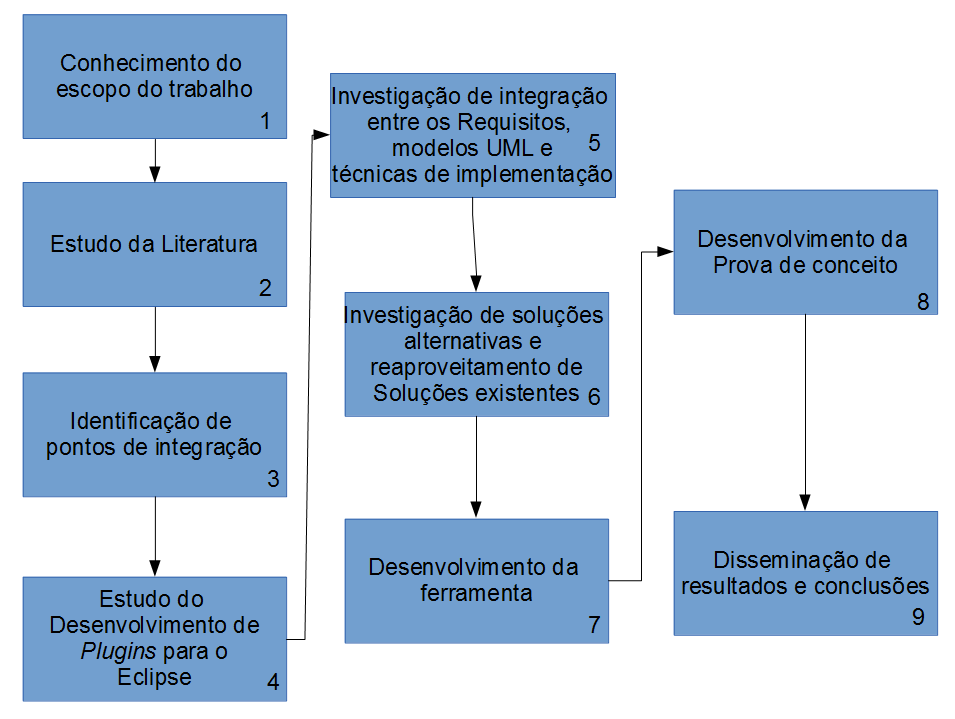
\includegraphics[scale=0.5]{./images/metodologia.png}
\caption{Etapas para a realiza��o deste trabalho}
\label{fig:metodologia}
\end{figure}

\section{Organiza��o do Trabalho}

Este trabalho est� organizado em seis cap�tulos. O primeiro cap�tulo
contextualizou a acessibilidade no desenvolvimento de \textit{sites}, apresentou
alguns desafios conhecidos na �rea e a motiva��o para o desenvolvimento do
mesmo.

O segundo cap�tulo apresenta os detalhes do dom�nio de acessibilidade na
\textit{Internet}. Esse cap�tulo apresenta as tecnologias e conceitos que devem
ser considerados para entregar produtos acess�veis. Tamb�m apresenta as
iniciativas e legisla��es acerca de acessibilidade de produtos \textit{web}.
Por fim, s�o apresentados os principais documentos, refer�ncias e diretrizes
para que os \textit{sites} sejam acess�veis.

O terceiro cap�tulo cont�m o levantamento bibliogr�fico realizado, com breves
descri��es de cada trabalho. O cap�tulo tem por objetivo mostrar qu�o amplo � o
dom�nio de acessibilidade na \textit{Internet}, bem como as propostas sugeridas
e os problemas ainda sem solu��o.

O quarto cap�tulo detalha o processo de integra��o de requisitos de
acessibilidade ao processo de desenvolvimento de \textit{software} (\gls{mta}), apresentando uma ferramenta para demonstrar como a integra��o ocorre.

O quinto cap�tulo apresenta uma prova de conceito, demonstrando a utiliza��o da ferramenta constru�da para a abordagem escolhida, bem como sua efetividade e limita��es.

O sexto e �ltimo cap�tulo apresenta as conclus�es gerais e trabalhos futuros.
\chapter{Acessibilidade na Web}

O modo de vida das pessoas come�ou a mudar radicalmente depois que Tim
Berners-Lee criou a \gls{www}, mais conhecida como
\textit{Web}. A \textit{Web} � um ambiente de documentos e dados interconectados globalmente
atrav�s da Internet \citep{mcpherson2009tim}. Em sua
concep��o inicial, a \textit{Web} foi explicitamente criada para poder ser utilizada sem o mouse, e
at� sem usar os olhos, se necess�rio \citep{thatcher:06}. Portanto, a maneira
como o usu�rio acessa um recurso na \textit{Web} pouco ou nada pode influenciar
na aquisi��o da informa��o.

A fim de tornar os \textit{sites} mais atrativos, v�rias tecnologias surgiram,
como \textit{JavaScript} \citep{goodman2001javascript} e \textit{Flash} \citep{adobe:12}.
Todavia, o uso indiscriminado dessas tecnologias podem, ao mesmo tempo, facilitar, inibir ou impedir o acesso aos
recursos de alguns usu�rios, principalmente dos usu�rios com algum tipo de
defici�ncia.

Obrigados por regulamenta��es e leis espec�ficas ou n�o, os desenvolvedores
gradualmente est�o adaptando seus \textit{sites} e produtos para as necessidades
dos usu�rios. O grande entrave para a dissemina��o da cultura de acessibilidade
na \textit{Web} est� na conscientiza��o dos desenvolvedores sobre a import�ncia
do tema, e sobre as consequ�ncias trazidas pela utiliza��o de tecnologias que se
tornam barreiras para o acesso ao conte�do disponibilizado na Web
\citep{freire:08,alves:11}.

O objetivo deste cap�tulo � apresentar os conceitos relevantes que devem ser
considerados para que os servi�os \textit{Web} entregues sejam acess�veis. Ser�o
apresentadas as tecnologias assistivas que auxiliam pessoas com defici�ncia, as
iniciativas para o desenvolvimento de sistemas \textit{Web} acess�veis, a
legisla��o e leis que asseguram a acessibilidade na \textit{Web}, as diretrizes que guiam o
desenvolvimento de produtos \textit{Web} acess�veis e quest�es referentes a
avalia��o de acessibilidade de produtos \textit{Web}.

\section{Tecnologias Assistivas e \textit{Design Universal}}

Pesquisadores da Universidade Estadual da Carolina do Norte definem
\textit{Design Universal} como o \textit{design} de produtos e ambientes us�veis por todas as pessoas, sem
precisar de adapta��es ou \textit{design} especializados. Tamb�m prop�em sete
princ�pios b�sicos para o \textit{design} de produtos, de forma  que esse
objetivo seja alcan�ado. S�o eles \citep{ncuniversity:11}:

\begin{itemize}
  \item utiliza��o equalit�ria: o produto � �til e
  comercializ�vel �s pessoas com diversas habilidades;
  \item utiliza��o flex�vel: o produto suporta uma grande variedade de
prefer�ncias individuais e habilidades;
  \item utiliza��o simples e intuitiva: o uso do produto � f�cil, independentemente da experi�ncia do usu�rio,
n�vel de conhecimento, compet�ncias lingu�sticas, ou educa��o;
  \item informa��o percept�vel: o produto transmite a informa��o
  necess�ria eficazmente para o utilizador, independentemente do ambiente,
condi��es ou habilidades sensoriais do usu�rio;
  \item toler�ncia a erros: o produto minimiza perigos e as
consequ�ncias adversas de a��es involunt�rias ou acidentais;
  \item esfor�o f�sico m�nimo: o produto pode ser usado de forma eficiente e
  confort�vel e com um m�nimo de fadiga;
  \item espa�o e tamanho adequado para aproxima��o e utiliza��o: o tamanho
  apropriado e o espa�o para utiliza��o do produto � suficiente para abordagem,
  alcance, manipula��o e uso independentemente do corpo do usu�rio; tamanho,
  postura ou mobilidade.
\end{itemize}

Esses princ�pios, obviamente, n�o s�o especificamente voltados para o
desenvolvimento de sistemas \textit{Web}, mas podem ser facilmente adaptados
para tal. Ainda assim, desenvolver sistemas \textit{Web} completamente
acess�veis � uma tarefa dif�cil. Deve-se considerar tamb�m que alguns dispositivos
s�o intrinsicamente inacess�veis para certos tipos de usu�rios, por exemplo, um
usu�rio cego n�o conseguir� extrair informa��es de um monitor tradicional.

Diante desse fato, � necess�rio fornecer aos usu�rios tecnologias intermedi�rias
para interceptar ou transformar a informa��o, apresentado-a de uma maneira que o
usu�rio consiga entender. Essas tecnologias s�o denominadas tecnologias
assistivas.
Tecnologia assistiva �, portanto, o conjunto de equipamentos, servi�os,
estrat�gias e pr�ticas concebidas para atenuar os problemas encontrados pelas pessoas com necessidades especiais \citep{cook:95}.

Existem diversos tipos de tecnologias assistivas, a escolha depende da
necessidade do usu�rio. � importante considerar que a dificuldade no acesso pode ser
permanente ou moment�nea. A seguir ser�o apresentadas algumas tecnologias
assistivas para certas defici�ncias:

\begin{itemize}
  \item Cegueira
  	\begin{itemize}
  	  \item Leitor de tela: software que l� o que est� na tela do computador e
  	  informa a sa�da, seja em um sintetizador de voz, ou um display \textit{braille}. Ex:
	  \textit{JAWS} \citep{freedom_jaws:13} e \textit{DOSVOX} \citep{nce-ufrj:13};
  	  \item Navegador textual: navegador que n�o carrega imagens. Deve ser usado
  	  em conjunto com o Leitor de Tela. Ex: \textit{Lynx} \citep{lynx:13}
  	  \item Navegador com voz: permite a navega��o por meio da voz. Ex:
  	  \textit{Opera} \citep{opera:13} e
  	  \textit{Firefox} com o plugin \textit{Text to Voice} \citep{ttv:13}
  	\end{itemize}
  \item Baixa vis�o
  	\begin{itemize}
  	  \item Ampliador de tela: software que amplia o conte�do da p�gina para
  	  facilitar a leitura. Ex:
  	  \textit{MAGic Screen Magnification} \citep{freedom_magic:13}
  	\end{itemize}
  \item Defici�ncia f�sica
  	\begin{itemize}
  	  \item \textit{Eye-tracking}: capta as a��es por meio do movimento dos
  	  olhos.
  	  Ex: \textit{LEA} \citep{lea:13}
  	  \item Teclado alternativo: dependendo da defici�ncia do usu�rio ou do
  	  dispositivo, um teclado alternativo pode ser inserido no contexto. Para deficientes visuais,
  	  teclados \textit{braille} s�o indicados \citep{4809825}. Para usu�rios com
  	  dispositivos m�veis, um teclado virtual pode ser a melhor solu��o
  	  \citep{5469165}.
  	\end{itemize}
  	\item Defici�ncia auditiva
  		\begin{itemize}
  		  \item Quando o usu�rio n�o perdeu 100\% da audi��o, ele pode usar softwares que melhoram o desempenho do �udio do computador. Mas o mais
  		  comum � a utiliza��o de legendas juntamente com as m�dias que possuem
  		  informa��es sonoras.
  		\end{itemize}
\end{itemize}

No momento da pesquisa n�o foram encontradas tecnologias assistivas para outros
tipos de defici�ncias.

\section{Legisla��o sobre acessibilidade na \textit{Internet}}

A primeira Lei sobre acessibilidade na \textit{Internet} foi a \textit{Section
508}, proposta em 1998 pelo Governo dos Estados Unidos \citep{section508:98}.
Segundo essa lei, a tecnologia inacess�vel interfere na capacidade individual de
adquirir e usar a informa��o de maneira r�pida e f�cil. A \textit{Section 508}
foi decretada para eliminar barreiras na tecnologia da informa��o,
disponibilizando novas oportunidades para as pessoas com necessidades especiais
e incentivando o desenvolvimento de tecnologias que as auxiliem a atingir esses
objetivos \citep{freire:08}.

Ap�s essa iniciativa, pa�ses em todo o mundo come�aram a incorporar t�picos de
acessibilidade no meio digital em suas leis j� existentes, ou at� mesmo
confeccionar novas. Por exemplo, a Lei \gls{dda}, institu�da pelo
governo brit�nico em 1995 \citep{dda:95}, foi alterada em 1999 e passou a possuir uma se��o especificamente sobre \textit{websites}
\citep{webcredible:11}. � v�lido mencionar que o ``n�vel'' de acessibilidade do
\textit{site} n�o � mencionado: o DDA requer que sejam realizadas ``adapta��es
razo�veis'' para garantir que uma pessoa com defici�ncia possa acessar o mesmo.

No Brasil, as Leis
10.048/2000 \citep{l10048:00} e
10.098/2000 \citep{l10098:00},
regulamentadas pelo Decreto
5.296/2004 \citep{d5296:04},
tornam obrigat�ria a acessibilidade nos websites da administra��o p�blica para o uso das pessoas com necessidades especiais para garantir o pleno acesso �s informa��es.

\section{Documentos e padr�es}

Existem dois grandes �rg�os que documentam e fornecem diversas especifica��es e
recomenda��es para os padr�es e novas tend�ncias da \textit{Internet}. Um deles
� o \gls{ietf} \citep{ietf:13} que tem
um car�ter mais arquitetural, preocupado principalmente com os protocolos e
recursos utilizados na \textit{Internet}. O outro � o \gls{w3c} \citep{w3c:13} que
tem um car�ter voltado para \textit{front end} e aplica��es. Este �ltimo possui
uma ramifica��o denominada \gls{wai} \citep{wai:13}, que se preocupa com as
quest�es referentes � acessibilidade na \textit{Internet}.

Quando se trata de padr�es e recomenda��es de acessibilidade na
\textit{Internet}, a \gls{w3c}-\gls{wai} � refer�ncia internacional. Todo
tipo de trabalho sobre acessibilidade na \textit{Internet} est�
relacionado (direta ou indiretamente) aos documentos da \gls{w3c}-\gls{wai}. A
Figura \ref{fig:relation} mostra quais documentos devem ser consultados pelos
desenvolvedores para atingir seus objetivos sobre acessibilidade.

\begin{figure}[h]
\centering
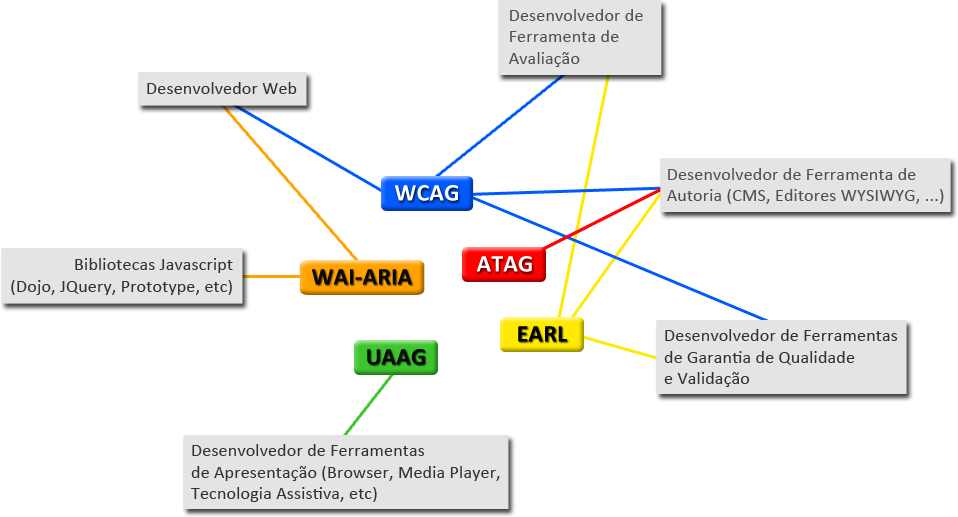
\includegraphics[scale=0.4]{./images/relation}
\caption{Rela��o de interesses entre os desenvolvedores e a documenta��o
\gls{w3c}-\gls{wai}: \gls{wcag}, \gls{atag}, \gls{wai-aria},
\gls{uaag} e \gls{earl}}
\label{fig:relation}
\end{figure}

A seguir, ser�o apresentados os cinco principais documentos de
refer�ncia publicados pela \gls{w3c}-\gls{wai}.

\subsection{WCAG}

O \gls{wcag} � um documento que
fornece diretrizes e recomenda��es para implementa��o de acessibilidade em
\textit{sites} \citep{wcagover:13}. A vers�o 1.0 do \gls{wcag} foi publicada em
1999 \citep{wcag10:13}. O documento � dividido em 14 diretrizes, cada uma com seus
respectivos \textit{checkpoints}.
Cada \textit{checkpoint} por sua vez possui uma prioridade.

As prioridades s�o divididas em grupos: as prioridades n�vel 1 (devem ser
atendidas), as prioridades n�vel 2 (deveriam ser atendidas) e as prioridades
n�vel 3 (poderiam ser atendidas). Se alguma prioridade n�vel 1 n�o for atendida,
um ou mais grupos de usu�rios ficar�o impossibilitados de acessar as informa��es
do documento. Se alguma prioridade n�vel 2 n�o for atendida, um ou mais grupos
de usu�rios ter�o dificuldades em acessar as informa��es em qualquer parte
documento.
Se alguma prioridade n�vel 3 n�o for atendida, um ou mais grupos de usu�rios ter�o
dificuldades em acessar alguma informa��o em partes espec�ficas do documento.

Se todos os \textit{checkpoints} com prioridade 1 forem atendidos, o documento
possui n�vel de conformidade ``A''. Se todos os \textit{checkpoints} com
prioridade 1 e 2 forem atendidos, o documento possui n�vel de conformidade
``AA''. Por fim, se todos os \textit{checkpoints} forem atendidos, o documento
possui o n�vel de prioridade ``AAA''. A Tabela \ref{tab:wcag} relaciona as
informa��es descritas at� agora para os n�veis de prioridade do \gls{wcag}
1.0.

\begin{table}[h]
\begin{center}
\begin{tabular}{|p{2cm}|p{4cm}|p{4cm}|p{4cm}|}%|c|c|c|c|}
\hline
\textbf{Prioridade} & \textbf{Recomenda��o} & \textbf{N�vel de Conformidade} &
\textbf{Impacto (para determinado grupo de usu�rios)} \\ \hline N�vel 1 &
devem ser atendidas & A (N�vel 1) & impossibilidade de acesso ao documento \\ \hline N�vel 2 & deveriam ser atendidas & AA (N�vel 1 e 2) & dificuldade no acesso ao documento \\ \hline
N�vel 3 & poderiam ser atendidas & AAA (N�vel 1, 2 e 3) & dificuldade no acesso
de partes espec�ficas do documento caso n�o seja atendida \\ \hline
\end{tabular}
\end{center}
\caption{N�veis de Conformidade do \gls{wcag} 1.0}
\label{tab:wcag}
\end{table}

Em 2008, o \gls{w3c}-\gls{wai} liberou a segunda vers�o do
\gls{wcag} \citep{wcag20:13}.
Segundo a \textit{WAI}, ``O \gls{wcag} 2.0 aplica-se amplamente a tecnologias mais avan�adas; � mais f�cil de usar e entender; �
precisamente validado com testes autom�ticos e avalia��o humana''. O documento possui 12 diretrizes, organizadas em 4
princ�pios:
percep��o, compreens�o, opera��o e robustez. Cada diretriz possui crit�rios de
sucesso test�veis, nas mesmas prioridades do \gls{wcag} 1.0. A \textit{WAI}
recomenda a utiliza��o do \gls{wcag} 2.0 e, devido �s semelhan�as com o
\gls{wcag} 1.0, sabe-se que a maioria dos sites em conformidade com o
\gls{wcag} 1.0 n�o requerem mudan�as significativas para estar em conformidade com o \gls{wcag} 2.0 e alguns nem mesmo necessitam de
mudan�as. As principais diferen�as podem ser vistas no site da \textit{WAI}, na
p�gina espec�fica sobre o assunto \citep{wcagdiff:13}. \citet{branco:09} fez um
breve comparativo dos dois documentos e constatou que a Tabela \ref{tab:wcag} � v�lida para o \gls{wcag} 2.0 e que, principalmente, as orienta��es de cada
\textit{guideline} se tornaram mais claras e f�ceis de testar.

� v�lido observar que nem todos os desenvolvedores concordam com as
diretrizes ou recomenda��es do \gls{wcag} 1.0 ou mesmo \gls{wcag} 2.0
\citep{clark:11}, apesar deste �ltimo ter se tornado um padr�o internacional
\citep{ISO:40500:2012}.
De fato, um grupo fechado de desenvolvedores preparou uma vers�o de extens�o/atualiza��o/corre��o n�o oficial do \gls{wcag} 1.0,
denominada \gls{wcag} Samurai \citep{wcagsamurai:11}.

Existem diversas diretrizes de acessibilidade, cada qual com suas
particularidades e voltadas para realidades espec�ficas. Alguns exemplos s�o:
\gls{clf}, substitu�da pelo documento \textit{Web Standards for the Government
of Canada}, do Canad� \citep{clf:13}, \gls{nda}, da Irlanda \citep{nda:13} e as diretrizes de \textit{design} de
acessibilidade da \textit{Microsoft} \citep{microsoft:09}.

O governo brasileiro possui um padr�o pr�prio, denominado \gls{emag}.
Atualmente na sua terceira vers�o \citep{emag:13}, o \gls{emag} � baseado no
\gls{wcag} 2.0, mas voltado para a realidade local. Em rela��o a vers�o anterior, o documento passou
por mudan�as sutis, por exemplo, a elimina��o das divis�es de vis�o t�cnica e vis�o do cidad�o. Apesar desse modelo poder ser usado em
outras iniciativas, � explicitado que o mesmo deve ser seguido para os
\textit{sites} governamentais. Por isso, n�o existem mais n�veis de prioridade
(todas as recomenda��es devem ser cumpridas) e uma se��o especial foi inclu�da
com o objetivo de padronizar elementos de acessibilidade que devem existir em
todos os \textit{sites} e portais governamentais.

\subsection{\textit{WAI-ARIA}}

Estamos em plena era da \textit{Web 2.0}, com \textit{sites} complexos e
din�micos e, consequentemente, controles da interface de usu�rio mais complexos
tamb�m. As tecnologias assistivas precisam interagir com esses controles para
que a experi�ncia de utiliza��o seja positiva para usu�rios com defici�ncia.
Contudo, as informa��es que as tecnologias assistivas necessitam para poder
manipular esses elementos complexos normalmente n�o est�o presentes na maioria
das tecnologias \textit{Web}.

Tecnologias \textit{Web 2.0} podem ser inacess�veis at� para usu�rios que n�o
possuem nenhum tipo de defici�ncia, mas possuem alguma barreira tecnol�gica, por exemplo, um menu
\textit{drag-and-drop} para o usu�rio que n�o possui um \textit{mouse}.
A atualiza��o de determinadas regi�es do \textit{site} pelas tecnologias citadas
tamb�m s�o um grande problema para as tecnologias assistivas (principalmente para o
\textit{Screen Reader}). Exemplos de tecnologias desse tipo s�o: \gls{ajax}
\citep{garrett:05} e \gls{dhtml} \citep{teague2001dhtml}.

O documento \gls{wai-aria} pretende
resolver esses desafios de acessibilidade definindo como a informa��o sobre a
funcionalidade do elemento deve ser entregue � tecnologia assistiva,
adicionando atributos, t�cnicas de navega��o, marca��o de regi�es, entre
outras \citep{ariaover:13}.

O \gls{wai-aria} �, portanto, um \textit{framework} que indica aos
desenvolvedores:

\begin{itemize}
  \item pap�is que descrevem o tipo do elemento apresentado;
  \item pap�is que descrevem a estrutura da p�gina;
  \item propriedades que descrevem o \textit{status} do elemento;
  \item propriedades que definem as ``regi�es vivas'' (din�micas);
  \item propriedades para elementos \textit{drag-and-drop};
  \item uma maneira para navegar e interagir com os elementos citados.
\end{itemize}

A documenta��o n�o est� inteiramente completa. Ao final do ano de 2011, a
vers�o definitiva do documento ainda n�o havia sido liberada. Como as
especifica��es do HTML 5 e do \gls{wai-aria} ainda n�o est�o
completamente definidas, algumas marca��es ficam sobrepostas
\citep{html5aria:11}. Contudo, desenvolvedores influentes afirmam que o padr�o
\gls{html}5 n�o vai tornar o uso do \gls{wai-aria} redundante
\citep{irish:11,faulkner:11}.

Esta documenta��o � voltada principalmente para desenvolvedores \textit{Web},
desenvolvedores de tecnologias \textit{Web 2.0} e desenvolvedores de
\textit{Javascript frameworks} como \textit{jQuery} \citep{jquery:13},
\textit{Dojo} \citep{dojo:13},
\textit{MooTools} \citep{mootools:13},
\textit{Prototype} \citep{prototype:13}, entre outros.

\subsection{\textit{ATAG}}

Ferramentas de Autoria s�o \textit{softwares} e
servi�os que permitem a qualquer pessoa produzir \textit{sites} e conte�do
\textit{web}. Esse tipo de ferramenta geralmente possui uma \textit{engine} que exibe o conte�do fornecido pelo
usu�rio utilizando padr�es e \textit{templates} previamente configurados
na ferramenta. Pela facilidade e rapidez de ``postar'' conte�do, muitos
us�arios (principalmente usu�rios leigos em computa��o) utilizam ferramentas desse tipo.

Existem v�rias ferramentas de autoria e cada uma tem sua
particularidade. Existem ferramentas para produ��o de \textit{blogs}, para
produ��o de portais chamadas \gls{cms}, de cria��o
de p�ginas \textit{wiki}, entre outras. Alguns exemplos de ferramentas
s�o: \textit{Wordpress} \citep{wordpress:13},
\textit{Joomla} \citep{joomla:13},
\textit{Drupal} \citep{drupal:13},
\textit{Plone} \citep{plone:13}, Sistemas
\textit{Wiki} \citep{wiki:13} e
\textit{Moodle} \citep{moodle:13}.

N�o raro, empresas e organiza��es desenvolvem suas pr�prias ferramentas de
autoria, principalmente quando o tipo de conte�do a ser postado � muito
espec�fico, ou quando a regra de neg�cios � diferente das ferramentas
convencionais. Pesquisadores e estudantes da Universidade Federal de Mato Grosso do Sul (UFMS) desenvolveram
ferramentas de autoria pr�pria, chamadas \textit{Titan} \citep{Carromeu:2010:CAE:1796182.1796987},
\textit{Pantaneiro} \citep{sandim:09} e \textit{Pantaneiro acess�vel}
\citep{maia:10}.

� um desafio prover total acessibilidade para o conte�do gerado por essas
ferramentas, visto que este � fornecido pelo usu�rio que normalmente �
leigo no assunto. A \gls{w3c}-\gls{wai} publicou um documento destinado a produ��o
de ferramentas de autoria, denominado
\gls{atag} \citep{atag:13} e o objetivo deste documento � definir como as
ferramentas de autoria deveriam ajudar os desenvolvedores a fornecer conte�do em conformidade com o \gls{wcag}. Mais do que isso, este documento explica
como tornar as ferramentas de autoria acess�veis para que pessoas com defici�ncia possam produzir seu pr�prio conte�do.

O documento \gls{atag}, assim como o \gls{wcag}, possui diretrizes e
\textit{checkpoints} para alcan�ar o resultado previsto. A vers�o 1.0, de
Fevereiro de 2000 \citep{atag10:13}, possui 28
\textit{checkpoints} e norteia o desenvolvimento de ferramentas de autoria levando em considera��o:

\begin{itemize}
  \item produzir o \textit{site} em conformidade com as diretrizes de
  acessibilidade;
  \item ajudar o usu�rio da ferramenta de autoria com informa��es relativas a
  acessibilidade do \textit{site};
  \item prover maneiras de checar e corrigir conte�do inacess�vel;
  \item integrar acessibilidade com ajuda, documenta��o e percep��o; e
  \item tornar a pr�pria ferramenta de autoria acess�vel para deficientes.
\end{itemize}

A vers�o 2.0 do documento ainda est� em
desenvolvimento \citep{atag20:13}. A novidade � que na nova vers�o, cada diretriz est�
relacionada a um princ�pio, percept�vel ao desenvolvedor.

O documento \gls{atag} � voltado principalmente para desenvolvedores de
ferramentas de autoria, incluindo:

\begin{itemize}
  \item ferramentas de edi��o \gls{wysiwyg};
  editores \gls{html} e \gls{xml});
  \item ferramentas que transformam documentos em formatos \textit{web} (por
  exemplo, transforma��o \textit{.doc} para \textit{.html});
  \item ferramenta de produ��o multim�dia \text{web} (ferramentas de autoria
  \gls{smil}) \citep{smil:13};
  \item ferramentas de publica��o e \gls{cms};
  \item ferramentas de gerenciamento de \textit{layout};
  \item qualquer ferramenta que permite aos usu�rios publicar e compartilhar
  conte�do.
\end{itemize}

\subsection{\textit{UAAG}}

As ferramentas que permitem ao usu�rio acessar o conte�do \textit{Web} s�o
chamadas \textit{User Agents}, ou Agentes de Usu�rio. Essas ferramentas incluem
navegadores, \textit{media players} e tecnologias assistivas.

A \gls{w3c}-\gls{wai} possui um documento voltado para os desenvolvedores de
\textit{User Agents} chamado
\gls{uaag} \citep{uaag:13}. A vers�o 1.0 do
documento, de Dezembro de
2002 \citep{uaag10:13}, possui 12 diretrizes de acessibilidade.
A vers�o 2.0 \citep{uaag20:13} ainda n�o foi finalizada.

O conjunto de \textit{checkpoints} que o \gls{uaag} 1.0 cobre s�o:

\begin{itemize}
  \item acesso a todo o conte�do, incluindo conte�do amarrado a eventos
  disparados por a��es de teclado e \textit{mouse};
  \item controle de usu�rio sobre a maneira como o conte�do �
  renderizado\footnote{Renderiza��o � o processo de gera��o de uma imagem
  por meio do processamento de um modelo computacional};
  \item controle de usu�rio sobre a interface, com informa��es sobre as
  caracter�sticas de acessibilidade;
  \item interface de programa��o padr�o, para prover intera��o com tecnologias
  assistivas.
\end{itemize}

\subsection{\textit{EARL}}

O documento \gls{earl} � na verdade um
formato definido para expressar resultados de testes, principalmente os
resultados gerados automaticamente por ferramentas de
avalia��o \citep{earl:13}.
Este documento utiliza \gls{rdf} \citep{rdf:13} para definir
os termos que expressar�o os resultados dos testes.

A vers�o 1.0 do documento ainda est� em
desenvolvimento \citep{earl10:13} e tem o objetivo de tratar os resultados de testes
das seguintes ferramentas:

\begin{itemize}
	\item ferramentas de avalia��o de acessibilidade;
	\item ferramentas de garantia de qualidade e valida��o;
	\item ferramentas de autoria e desenvolvimento; e
	\item descri��o de conte�do Web.
\end{itemize}

\section{Considera��es Finais}

Neste cap�tulo foram apresentados a legisla��o, documentos e tecnologias de
maior relev�ncia para o contexto de acessibilidade na \textit{Web}. O pr�ximo cap�tulo apresenta a pesquisa bibliogr�fica realizada neste trabalho.
\chapter{Pesquisa Bibliogr�fica}

Para realizar este trabalho, uma pesquisa bibliogr�fica foi executada com o
intuito de verificar as principais �reas de interesse no assunto, bem como a
motiva��o dos pesquisadores e os resultados alcan�ados. Os artigos estudados
levaram em conta o assunto de acessibilidade no contexto de Engenharia de
\textit{Software}, destacando-se algumas fases e atividades do processo de
desenvolvimento de \textit{software} indicados a seguir:

\begin{itemize}
  \item Requisitos
  \item Arquitetura
  \item Navega��o
  \item Interface
  \item Conte�do
  \item Avalia��o
\end{itemize}

Foram analisadas tamb�m \textit{surveys} que indicavam o estado da arte e da
pr�tica em rela��o ao assunto.

Os resultados da pesquisa bibliogr�fica s�o apresentados a seguir. Para melhor
entendimento, os artigos est�o organizados em se��es de acordo com os itens
descritos anteriormente (alguns artigos poderiam ser encaixados em mais de um
item, dessa forma optou-se por deixar no item de maior rela��o com
este trabalho).

\section{Requisitos}

\cite{Trewin:2010:ACT:1805986.1806029} realizaram uma pesquisa
com os desenvolvedores da \textit{IBM} com o objetivo da pesquisa foi
verificar como as ferramentas de apoio a acessibilidade podem ajudar os desenvolvedores.
Quando acessibilidade � envolvida no projeto, algumas estat�sticas de
consumo de tempo foram levantadas nas etapas.

Os desenvolvedores explicaram que as ferramentas atuais de apoio a
acessibilidade atrapalham o desenvolvimento, tornando o processo moroso.
Quest�es importantes sobre as ferramentas de apoio foram levantadas, tais como:

\begin{itemize}
  \item Quais funcionalidades a ferramenta de apoio deve oferecer?
  \item A ferramenta de apoio deve ou n�o ser integrada � ferramenta de
  desenvolvimento?
\end{itemize}

A pesquisa constatou que o \textit{design}, testes e encontrar solu��es
tecnol�gicas para o problema s�o os aspectos mais dif�ceis para se produzir uma
aplica��o \textit{web} acess�vel. A pesquisa mostrou tamb�m que os desenvolvedores
n�o confiam completamente nos resultados fornecidos pelas pelas ferramentas de
testes, por causa dos falsos positivos, al�m de mencionar que as explica��es
fornecidas pelas ferramentas n�o suficientemente detalhadas.

\cite{analuizadias:2010} estudaram o est�gio da
inser��o de acessibilidade nas etapas de desenvolvimento de \textit{software}.
Para isso, foram buscados artigos nos portais \textit{Springer, ACM,
IEEE, Elsevier, Wiley e Scielo}.

Os artigos relevantes foram classificados de acordo com a norma \textit{ISO/IEC
12207:1998} (Requisitos, Projeto, Constru��o, etc) \citep{iso12207:98}. Uma das
observa��es dos autores � que a maioria das pesquisas se refere a testes com
usu�rios, enquanto nenhuma contempla instala��o de \textit{software}. Esta � uma
constata��o interessante, visto que usu�rios com defici�ncia visual conseguem
instalar completamente um sistema operacional
\textit{Linux}\footnote{https://help.ubuntu.com/community/Accessibility
e http://www.linuxacessivel.org/}, mas h� v�rios requisitos anteriores que devem ser considerados para que o usu�rio consiga executar a tarefa de forma adequada (por exemplo, baixar a imagem do Sistema Operacional e gravar em um CD/DVD ou
\textit{pen drive}). Nada foi encontrado na literatura sobre a instala��o de
outros sistemas operacionais (por exemplo, \textit{Windows}) por deficientes
visuais.

\cite{4756193} prop�s uma ferramenta para
especifica��o de requisitos de acessibilidade. Sua proposta � unir os
requisitos das diretrizes de acessibilidade com os requerimentos da engenharia
de \textit{software} tradicional, incluindo requerimentos espec�ficos de
acessibilidade no Documento de Requisitos. O trabalho � baseado nos \textit{checklists} e \textit{checkpoints}
das diretrizes de acessibilidade mais conhecidas. 
 
A ferramenta, nomeada \textit{AccessOnto}, aproveita a sa�da de algumas
ferramentas \textit{CASE} tais como
\textit{SELECT}\footnote{http://www.selectbs.com/analysis-and-design/select-architect}
e prev� integra��o com o \textit{IBM Rational Policy Tester
Accessibility}\footnote{http://www-01.ibm.com/software/awdtools/tester/policy/accessibility/}.
Um \textit{XML Schema} prov� as descri��es, regras e classes, descrevendo as diretrizes, caracter�sticas do usu�rio e
objetos no ambiente de intera��o. A ferramenta � usada para intervir em
diagramas de caso de uso, diagramas de classes e diagramas de transi��o de
estados.

\cite{4196334} discutiram as iniciativas de
padroniza��o de acessibilidade no dom�nio \textit{e-Learning}. De acordo com os
autores, h� muitas institui��es trabalhando na padroniza��o de tecnologias
\textit{e-Learning}, nos seguintes subdom�nios: metadados, agrega��o de
conte�do, informa��es do estudante, acessibilidade e \textit{Runtime}.

Os autores aprofundaram seus estudos nos padr�es \gls{lip}, \gls{acclip} e
\gls{accmd}\footnote{http://wiki.cetis.ac.uk/ACCMD\_Briefing}, propostos pela
\gls{ims}\footnote{http://www.imsglobal.org/accessibility/}, e explicaram a
proposta de \gls{dp}, estendendo os padr�es mencionados.

\cite{5260918} estudaram os princ�pios e conceitos de
acessibilidade em \textit{sites} educacionais. Os autores descrevem a
heteogeneidade dos estudantes (quest�es como defici�ncias, equipamentos,
habilidades, idade, entre outras). Os autores sugerem que alguns princ�pios de \textit{design} devem ser assumidos
(flexibilidade, simplicidade e toler�ncia a erros. Tamb�m sugerem
aplicar um processo de desenvolvimento \textit{top-down} (Defini��o $>$ An�lise $>$ Prot�tipo $>$ Testes $>$ Integra��o $>$ Libera��o e
Manuten��o) para atingir os objetivos e prover um produto acess�vel.

\cite{springerlink:10.1007/978-3-642-02713-0_67} estudaram como incorporar acessibilidade junto a
an�lise de requisitos. Uma pesquisa inicial foi feita para verificar em que
est�gio de desenvolvimento a acessibilidade � considerada e quanto tempo �
dedicado a esse fim. H� uma discuss�o se requisitos de acessibilidade devem
ser considerados requisitos funcionais ou requisitos n�o funcionais, j� que
alguns autores consideram acessibilidade como uma sub-�rea de usabilidade.

Os autores trataram requisitos de acessibilidade como requisitos n�o funcionais,
utilizando como base o \textit{NRF Framework}, que representa o requisito n�o
funcional atrav�s de operacionaliza��es est�ticas e din�micas, transformando a
representa��o em um grafo \citep{Cysneiros:2001:UUR:782096.782098} e tratando
os requisitos como objetivos (\textit{goal graph}), que precisam ser
satisfeitos. No trabalho de \citet{springerlink:10.1007/978-3-642-02713-0_67},
altera��es no \gls{nfr} \textit{goal graph} foram feitas, transformando-o em um
\gls{ar} \textit{graph}. O diagrama de casos de uso � alterado para comportar a acessibilidade.

\cite{Akhter:2009:CFE:1632189.1632275} propuseram um \textit{framework}
conceitual para aumentar a confian�a de \textit{sites} por usu�rios que utilizam leitores de tela. Algumas diretrizes s�o propostas, tais como:
\begin{itemize}
  \item informar que o usu�rio est� em uma p�gina segura (\gls{https});
  \item apresentar, assim que poss�vel, informa��es sobre certificados e, se
  necess�rio, duplicar a informa��o;
  \item informar imediatamente se uma p�gina � recarregada, poss�vel atrav�s
  de regi�es \gls{wai-aria}.
\end{itemize}

\section{Arquitetura}

\cite{Fuertes:2011:DHW:1969289.1969294} apresentaram o projeto da
ferramenta \textit{Hera-FFX}, um plugin para o navegador \textit{Firefox}. O
projeto tem por objetivo eliminar as limita��es da ferramenta \textit{Hera 1.0}
\footnote{http://www.sidar.org/hera/} e estender sua funcionalidade, realizando as avalia��es
utilizando o \gls{wcag} 2.0.

O trabalho � interessante por fazer compara��es com outras ferramentas de
avalia��o, e mostrar quais caracter�sticas seriam desej�veis que uma
ferramenta desse tipo contivesse. Dentre estas caracter�sticas, podem ser
citadas:

\begin{itemize}
  \item avalia��o preliminar autom�tica;
  \item suporte para preenchimento manual;
  \item modifica��o da p�gina de apresenta��o
  \item exibi��o do c�digo anotado;
  \item avalia��o de p�ginas locais;
  \item avalia��o de p�ginas com acesso restrito;
  \item avalia��o de renderiza��o de p�ginas;
  \item gera��o de relat�rios;
  \item suporte para treinamento;
  \item capacidade de multi-sess�o;
  \item flexibilidade.
\end{itemize}

\cite{Bigham:2010:ADE:1878803.1878812} propuseram uma ferramenta em que usu�rios
finais apontem problemas de acessibilidade. A ferramenta � uma extens�o do leitor de tela
\textit{WebAnywhere}\footnote{http://webanywhere.cs.washington.edu/}. Um script \textit{server-side} guarda o conjunto de a��es de usu�rio,
permitindo ao desenvolvedor reproduzi-las posteriormente. Essa ferramenta � �til
para compensar a defici�ncia das ferramentas de avalia��o autom�tica, que n�o
conseguem resolver completamente os problemas presentes no \textit{site}.

\cite{5564560} estudaram acessibilidade envolvendo
\textit{web services}. O estudo � baseado na forma como os \textit{web services}
se comunicam, atrav�s do protocolo
\textit{SOAP}\footnote{http://www.w3.org/TR/2003/REC-soap12-part0-20030624/}. Antes de entregar o conte�do, o \textit{web service} ``desempacota'' o mesmo e
analisa utilizando as diretrizes \gls{wcag}. Por esse motivo, as
funcionalidades s�o definidas em classes, assim como os n�veis de conformidade
do \gls{wcag}. Um m�dulo de valida��o foi desenvolvido, gerando relat�rios
\gls{earl}.

\cite{Schaik:2008:MUE:1367153.1367461} estudaram
a percep��o do usu�rio em rela��o � qualidade de \textit{sites} na internet. Foi
realizada uma pesquisa para verificar a percep��o do usu�rio com alguns \textit{sites} pr�-definidos. Os elementos do \textit{site} eram
reordenados e seu layout foi modificado. Dessa maneira, os usu�rios davam
seu parecer antes e depois da utiliza��o do mesmo.

A pesquisa considerou alguns princ�pios b�sicos, como beleza e qualidade,
tratando-os como vari�veis aleat�rias para proceder com o estudo estat�stico. O
estudo mostrou que a vari�vel aleat�ria \textit{beleza} � mais est�vel do que,
por exemplo, a percep��o do usu�rio sobre qualidade. A base de conhecimento
resultante pode ser usada para produzir um guia de \textit{design} na forma de
padr�es de \textit{design} para facilitar a compreens�o e aplica��o.

\cite{Buzzi:2008:MWE:1463160.1463210} propuseram modifica��es na \textit{Wikipedia} de forma
que a mesma se torne acess�vel para contribui��o de usu�rios cegos.

Os objetivos foram alcan�ados atrav�s das seguintes altera��es:
\begin{itemize}
  \item utiliza��o de regi�es \gls{wai-aria}, principalmente para
quest�es como foco nos elementos;
  \item altera��o da barra de ferramentas (de \textit{javascript} para
\gls{xhtml});
  \item mudan�a na forma de escolha de s�mbolos especiais.
\end{itemize}

\section{Navega��o}

\cite{5358165} constru�ram um \textit{plugin}
para \textit{NetBeans} que simula algumas defici�ncias visuais, para testar
principalmente aplica��es \textit{Java Swing}.

Os autores mencionam que existem v�rios simuladores de defici�ncias f�sicas na
literatura, sendo que o simulador proposto por eles cobre v�rios tipos de
defici�ncia visual (tais como catarata, hipermetropia, entre outras). Os resultados obtidos foram comparados com outros
simuladores da mesma categoria. A implementa��o foi projetada usando um design
centrado no usu�rio, justamente para entender suas maiores dificuldades.

\cite{4437943} propuseram a personaliza��o da
interface do usu�rio, tornando assim o conte�do acess�vel. A proposta permite
que os usu�rios definam como o conte�do deve ser apresentado. Os requisitos que devem ser considerados para alcan�ar esse grau de
flexibilidade s�o:
apresenta��o do conte�do, navega��o e busca. Como exemplo, os autores demonstraram as possibilidades da
abordagem montando uma linguagem descritiva em
\gls{javacc}\footnote{http://javacc.java.net/} para m�dia
\gls{rss}\footnote{http://www.rss-specifications.com/rss-specifications.htm}.

Os autores detalharam como a transforma��o ocorre
\citep{Encelle:2007:PUI:1243441.1243459}, usando
\gls{xpath}\footnote{http://www.w3schools.com/xpath/ xpath\_intro.asp},
\gls{smil} e \gls{xslt}\footnote{http://www.w3.org/TR/xslt}. Segundo os
autores, � relativamente simples utilizar a proposta sugerida, bastando apenas 3
utiliza��es para o usu�rio conseguir aprender a usar ferramenta e personalizar a interface que estiver usando.

\cite{Ferres:2007:IAS:1296843.1296857} propuseram um
m�todo para tornar gr�ficos acess�veis. A acessibilidade � alcan�ada da seguinte
maneira: os gr�ficos s�o confeccionados no \textit{Excel}, atrav�s de um \textit{plugin} feito para esse fim. Depois de publicado, um \textit{plugin} instalado no
navegador reconhece o gr�fico acess�vel, fornecendo a intera��o necess�ria para que o
usu�rio consiga extrair toda a informa��o necess�ria.

A navega��o no gr�fico foi inspirada em leitores de tela, portanto � feita
atrav�s do teclado. Al�m disso, o \textit{software} de leitura do gr�fico possui
um sintetizador de voz embutido.

\cite{Michail:2007:ABS:1547550.1547666} propuseram a
personaliza��o da navega��o nativa dos \textit{sites}, de acordo com as
prefer�ncias do usu�rio, atrav�s de um \textit{framework} que estende o
\textit{SeEBrowser}\footnote{http://seebrowser.it.teithe.gr/?q=en/node/32}. O
framework permite guardar anota��es de acessibilidade atrav�s de comandos
\textit{POST} e \textit{GET} do protocolo \gls{http}. As anota��es s�o
armazenadas no formato \gls{rdf}.

O \textit{software} possui algumas m�tricas para avaliar o n�vel dos atalhos
fornecidos ao usu�rio, contando pressionamento das teclas, tempo gasto em cada
p�gina, entre outras. A navega��o � reordenada baseada na relev�ncia das
informa��es previamente cadastradas, atrav�s das estat�sticas coletadas.

\section{Interface}

\textbf{\cite{5338903} propuseram a possibilidade de customiza��o
das interfaces de aplicativos \textit{web} (baseados em \gls{html} e
\gls{css}) de celulares de acordo com as prefer�ncias do usu�rio. O grande diferencial dessa proposta � que, utilizando \textit{Java Card} e
\gls{j2me}, as prefer�ncias s�o gravadas no \textit{chip SIM}, e n�o na
mem�ria do celular, como a maioria das aplica��es fazem. Dessa forma, � poss�vel
alterar o aparelho f�sico, mas as informa��es da interface n�o s�o perdidas.}

\cite{Pauwels:2009:EPO:1618879.1619082} questionaram a
melhor forma de evidenciar campos obrigat�rios em formul�rios. V�rios
pesquisadores afirmam que campos obrigat�rios de um formul�rio devem aparecer
logo no in�cio, destacados. A \textit{Apple} prefere a abordagem de usar
asteriscos, e s� destacar os campos que o usu�rio errou ap�s o usu�rio
submeter a a��o.

Em termos de acessibilidade, a pesquisa mostra que a abordagem de campos
coloridos � melhor do que a de asterisco, mas leitores de tela n�o s�o sens�veis a esse contexto.
Aparentemente, � bom utilizar as duas abordagens. Apesar disso, os autores n�o conseguiram
concluir qual cor deve ser utilizada, informando apenas que a cor utilizada para
seus testes foi a amarela.

\cite{Halbach:2010:TCA:1747589.1747607} tratou da
defici�ncia cognitiva (problemas com foco, dificuldade de leitura, entendimento,
mem�ria, entre outros). Os documentos \gls{wcag} 1.0 e 2.0 cobrem uma �rea
limitada dos problemas que a defici�ncia cognitiva podem trazer. Portanto, o autor prop�e um conjunto de princ�pios de \textit{design} para cada sub-�rea
e desenvolveu uma solu��o baseada no estudo de caso do
\textit{site} de servi�os p�blicos da Noruega. Nesse \textit{site}, 33\% dos chamados do \textit{Help
Desk} eram relativos a tela de \textit{login}. A solu��o apresentada �
interessante pois usa padr�es de \textit{design} pouco usuais em desenvolvimento
de \textit{sites}, por exemplo, usar uma �rea para informar o que o usu�rio
est� fazendo no momento, e quais s�o os pr�ximos passos. Isso auxilia pessoas
com problemas de m�moria, principalmente idosos.

\section{Conte�do}

\cite{Ferretti:2008:EYW:1368044.1368070} propuseram, atrav�s de objetos
\gls{accmd}, uma forma
compartilhada de prover acessibilidade em ambientes \textit{e-Learning 2.0}, principalmente para objetos multim�dia
\gls{smil}.

No ambiente virtual, o tutor disponibiliza o conte�do, que depois pode ser
acrescido de recursos pelas partes interessadas (tutor, estudantes, etc). A
edi��o colaborativa � feita por uma interface \textit{wiki-like}, na qual as
``camadas'' de acessibilidade s�o adicionadas aos objetos de aprendizagem, sob
supervis�o do tutor.

\cite{MartinGarcia:2009:PAE:1535654.1535665} estudaram a rela��o entre os \textit{Prosumers} (usu�rios
geralmente leigos que utilizam ferramentas de autoria para publicar
informa��es \textit{online}) e acessibilidade do conte�do
por eles disponibilizado. Deve ser levado em conta que
\textit{Prosumers} n�o s�o profissionais em constru��o de
\textit{sites}, muito menos em acessibilidade.

A inclus�o de acessibilidade no \gls{ugc} deve ser
feita, portanto, de forma transparente ao \textit{prosumer}.
Os autores explicitam algumas formas de tornar esse processo poss�vel:

\begin{itemize}
  \item acessibilidade orientada a plataforma (restri��o na gera��o, utiliza��o
  de templates, etc);
  \item acessibilidade dependente do criador (permitir a ferramenta ``sugerir''
  as quest�es de acessibilidade);
  \item acessibilidade auxiliada pela comunidade (treinamentos, compartilhamento
  de autoria, modera��o, etc).
\end{itemize}

\section{Avalia��o}

\cite{Vigo:2011:AWA:1963660.1963798} trataram de
quest�es relativas a m�tricas de acessibilidade. Existem muitas m�tricas propostas na literatura, tais como
\gls{uwem} \citep{cluster2:09}, \gls{waqm} \citep{vigo:07}, \textit{A3}
\citep{buhler:06}, \textit{$T^1$} \citep{t1:09}, \gls{wab} \citep{martinez:09},
\gls{pm} \citep{4380248}, entre outras. Os autores questionam qual � a
``qualidade'' de cada uma delas. Por qualidade, pode-se considerar a validade, confiabilidade, sensibilidade,
complexidade, entre outros par�metros. Esses par�metros devem ser considerados
para determinar em que cen�rio elas devem ser usadas (validadores desktop,
validadores \textit{online}, \textit{engine} de busca, etc). O motor de busca do \textit{Google} j� utiliza m�tricas de acessibilidade
para ``rankear'' os sites (essa m�trica n�o � de conhecimento p�blico)
\footnote{http://www.google.com/accessibility/labs/search/}.

Algumas m�tricas s�o dif�ceis de implementar e testar por ferramentas
autom�ticas. Os autores refor�am que h� v�rios aspectos que devem ser levados em
conta ao realizar um estudo comparativo entre as m�tricas. Contudo, mesmo
estando abaixo de um comportamento �timo, \textbf{as m�tricas apresentadas na literatura
que tiveram melhor comportamento em rela��o a (\ldots) foram}: \gls{waqm}, \gls{pm} e \gls{wab}.

\cite{Brajnik:2009:VRW:1639642.1639666} questionou a
validade das diretrizes de acessibilidade. O principal questionamento do
trabalho �: um mesmo conjunto de diretrizes de acessibilidade produzir� os mesmos resultados, se conduzido por pessoas ou
ferramentas diferentes?

Mesmo que a resposta para a pergunta anterior seja positiva, pode-se
perguntar qual � a qualidade dos m�todos de avalia��o utilizados e o qu�o
``test�veis'' s�o as diretrizes de acessibilidade.

O autor concluiu que as diretrizes do \gls{wcag} 1.0 s�o mais confi�veis do
que as diretrizes do \gls{wcag} 2.0. \textbf{Ainda assim, a confiabilidade n�o passou
dos 80\%
}.

\textbf{Texto do Andr�}
\section{MTA - Modelo de Tarefas de Acessibilidade}\label{chapter:mta}

\citet{Melo:2006:DPI:1298023.1298026} consideram importante apoiar o
desenvolvimento de sistemas acess�veis utilizando m�todos e t�cnicas que possam
explicit�-los e represent�-los. Com o objetivo de amparar o desenvolvimento de
softwares seguindo padr�es e \textit{frameworks} de desenvolvimento j� existentes, \citet{maia:10} prop�s o
MTA (Modelo de Tarefas de Acessibilidade).

O modelo proposto sugere tarefas de acessibilidade a serem empregadas nos
subprocessos do Processo de Desenvolvimento da Norma ISO/IEC
12207\footnote{Acess�vel em
http://www.iso.org/iso/catalogue\_detail?csnumber=43447}. A proposta apresentada
� que, alterando e adaptando esses subprocessos espec�ficos, a acessibilidade
do produto final seja melhorada.

\subsection{ISO/IEC 12207}

A norma ISO/IEC 12007 \citep{ieeeeia12207:1998} tem como objetivo prover um
padr�o para desenvolvimento e acompanhamento dos processos do ciclo de vida de
softwares. Os processos s�o separados por fundamentais, de apoio,
organizacionais e de adapta��o.

Os processos s�o divididos em atividades ou subprocessos e esses, por sua vez,
s�o divididos em tarefas. � importante mencionar que a norma n�o descreve as
t�cnicas espec�ficas utilizadas para a realiza��o das atividades, mas sim um
\textit{framework} de tal forma que � poss�vel planejar e entender o processo de
desenvolvimento do software.

Apesar de a norma poder ser utilizada parcialmente, algumas atividades dos
processos se relacionam com outros processos. Pode-se citar, por exemplo, tarefas do Processo de
Desenvolvimento que requeiram a documenta�a� de suas sa�das, e portanto, o
Processo de Documenta��o deveria ser utilizado \citep{maia:10}.

O MTA foi desenvolvido focado no Processo de Desenvolvimento. Neste processo,
encontram-se os seguintes subprocessos:

\begin{enumerate}
  \item Elicia��o dos requisitos do sistema;
  \item An�lise dos requisitos do sistema;
  \item Projeto Arquitetural do sistema;
  \item An�lise de Requisitos do software;
  \item Projeto de software;
  \item Constru��o do software (c�digo e teste de unidade);
  \item Integra��o do software;
  \item Teste do software;
  \item Integra��o do sistema; e
  \item Teste do sistema.
\end{enumerate}

\subsection{MTA integrado ao Processo de Desenvolvimento - ISO/IEC 12007}

Em cada subprocesso do Processo de Desenvolvimento, foram inseridas uma ou mais
tarefas de acessibilidade. A tabela \ref{table:isomta} relaciona os subprocessos
e as tarefas de acessibilidade relacionadas. \citet{maia:10} descreve os
subprocessos e como as tarefas de acessibilidade devem ser desenvolvidas.

\begin{table}[htbp]
\begin{center}
\tiny
\begin{tabular}{|l|l|}
\hline
\textbf{Subprocessos} & \textbf{Tarefas de acessibilidade} \\ \hline
1. Elicita��o dos requisitos do sistema & 1.1 Identificar os requisitos de
acessibilidade do sistema \\ \hline \multicolumn{ 1}{|l|}{2. An�lise de
requisitos do sistema} & 2.1 Especificar os requisitos de acessibilidade do sistema \\ \cline{ 2- 2} \multicolumn{ 1}{|l|}{}
& 2.2 Avaliar os requisitos de acessibilidade do sistema \\ \hline \multicolumn{
1}{|l|}{3. Projeto arquitetural do sistema} & 3.1 Alocar os requisitos de
acessibilidade aos elementos do sistema \\ \cline{ 2- 2} \multicolumn{ 1}{|l|}{}
& 3.2 Avaliar o projeto arquitetural do sistema com rela��o aos requisitos de
acessibilidade \\ \hline \multicolumn{ 1}{|l|}{4. An�lise de requisitos do
software} & 4.1 Estabelecer os requisitos de acessibilidade do software \\
\cline{ 2- 2} \multicolumn{ 1}{|l|}{} & 4.2 Avaliar os requisitos de
acessibilidade do software \\ \hline \multicolumn{ 1}{|l|}{5. Projeto de
software} & 5.1 Projetar as interfaces externas acess�veis \\ \cline{ 2- 2}
\multicolumn{ 1}{|l|}{} & 5.2 Realizar o projeto navegacional acess�vel \\
\cline{ 2- 2} \multicolumn{ 1}{|l|}{} & 5.3 Avaliar acessibilidade do projeto de
software \\ \hline \multicolumn{ 1}{|l|}{6. Constru��o do Software
(c�digo e teste de unidade)} & 6.1 Especificar t�cnicas para implementa��o da
acessibilidade da interface e do c�digo \\ \cline{ 2- 2}
\multicolumn{ 1}{|l|}{} & 6.2 Codificar cada unidade de software de acordo com
as t�cnicas de acessibilidade \\ \cline{ 2- 2}
\multicolumn{ 1}{|l|}{} & 6.3 Planejar teste de acessibilidade para cada unidade
de software \\ \cline{ 2- 2} \multicolumn{ 1}{|l|}{} & 6.4 Executar testes de
acessibilidade de cada unidade de software \\ \hline 7. Integra��o do software &
7.1 Planejar teste de acessibilidade do software integrado \\ \hline
\multicolumn{ 1}{|l|}{8. Teste do software} & 8.1 Conduzir testes de
acessibilidade do software \\ \cline{ 2- 2} \multicolumn{ 1}{|l|}{} & 8.2
Avaliar o resultado do teste de acessibilidade \\ \hline \multicolumn{
1}{|l|}{9. Integra��o do sistema} & 9.1 Realizar testes de acessibilidade no
sistema \\ \cline{ 2- 2} \multicolumn{ 1}{|l|}{} & 9.2 Avaliar os resultados dos
testes de acessibilidade do sistema \\ \hline 10. Teste do sistema & 10.1
Certificar a conformidade com os requisitos do sistema \\
\hline
\end{tabular}
\end{center}
\caption{Subprocessos e tarefas de acessibilidade do MTA}
\label{table:isomta}
\end{table}

\chapter{Desenvolvimento}

O MTA, como extens�o de um processo de desenvolvimento de \textit{software}, n�o
especifica qual � a maneira correta de executar as tarefas e atividades
propostas. � um desafio partir dos requisitos de acessibilidade e conseguir
entregar um produto acess�vel. Por isso, � fundamental haver um m�todo de
rastreabilidade desses requisitos, de forma que exista uma garantia de que a
implementa��o est� sendo feito de forma correta.

Os requisitos de acessibilidade devem ser propagados desde o in�cio do processo
(levantamento e confec��o do documento de requisitos) at� as etapas finais de
codifica��o e testes de forma consistente.

Para o trabalho proposto, definimos como escopo apenas os subprocessos 4
(An�lise de Requisitos de Software), 5 (Projeto de Software) e 6 (Constru��o do
Software) e suas respectivas tarefas de acessibilidade. Essa abordagem foi adotada pois, embora as defini��es de acessibilidade j�
come�am no subprocesso 1, � no subprocesso 4 que os requisitos s�o ``lapidados''
e o artefato de entrada das fases de projeto � gerado.

As tarefas de testes,
presentes no subprocesso 6, n�o ser�o levadas em considera��o.

A seguir, ser�o apresentados os relacionamentos entre os subprocessos citados
com o rastreio dos requisitos de acessibilidade.

\section{Subprocesso 4 - An�lise de Requisitos de Software}
\label{linktocase}

O especialista em acessibilidade � fundamental em todas as etapas descritas a
seguir, como j� refor�a o modelo MTA. Ele deve ter a experi�ncia e maturidade
para capturar os requisitos de acessibilidade no momento conveniente. Isso pode
ocorrer (e � desej�vel) no levantamento de requisitos de forma expl�cita
(sugerindo possivelmente um requisito funcional), de forma gen�rica e n�o
espec�fica (sugerindo possivelmente um requisito n�o funcional). O requisito de
acessibilidade pode n�o ser encontrado explicitamente neste momento, mas o
encontro posterir exigir� um refatoramento do modelo.

Requisitos funcionais e n�o funcionais s�o abordados no subprocesso 4, ponto de
partida deste trabalho no modelo MTA. Caso os requisitos n�o sejam identificados
nesta etapa, o especialista de acessibilidade dever�, no subprocesso 5,
especificar nos projetos de interface e navega��o os itens que merecem um
tratamento de acessibilidade espec�fico.

O objetivo do subprocesso 4 � estabelecer os requisitos dos elementos de
software do sistema. Elementos aqui s�o considerados interface e c�digo
\citep{maia:10}.

O MTA insere duas tarefas de acessibilidade, conforme mostrado na figura
\ref{fig:sub4}.

\begin{figure}[ht] \centering
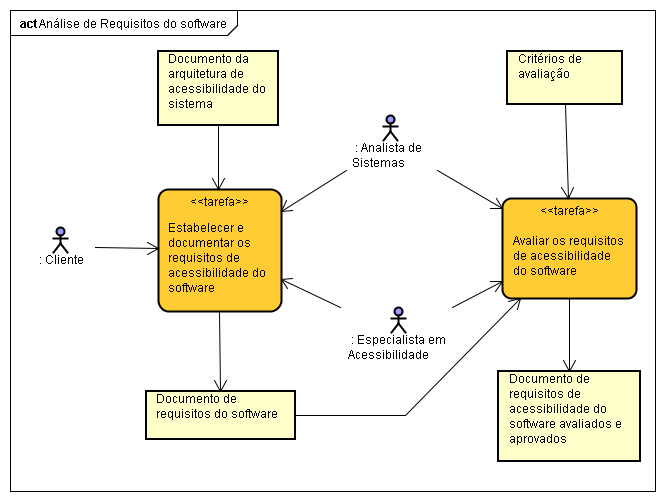
\includegraphics[width=.8\textwidth,height=200px]{./images/subprocesso4.png}
\caption{Tarefas para o subprocesso de an�lise de requisitos do software
\citep{maia:10}}
\label{fig:sub4}
\end{figure}

� importante ressaltar que os requisitos j� s�o parcialmente coletados em
subprocessos anteriores, mas � apenas nesse subprocesso que os requisitos de
interface e c�digo s�o considerados. � nesse subprocesso tamb�m que ir� originar
o artefato para as fases de projeto e codifica��o.

 A sa�da da tarefa \textbf{Avaliar os requisitos de acessibilidade de software}
 (Documento de requisitos de acessibilidade do software avaliados e aprovados)
 � processada, gerando um novo artefato. A proposta � que mais um
 artefato seja gerado, sendo um documento de requisitos em um formato leg�vel
 por m�quina, n�o ambiguo e que possa ser gerenciado por uma ferramenta
 \gls{case}, que ser� utilizado nos passos subsequentes para rastreamento dos
 requisitos de acessibilidade. A escolha adotada neste trabalho � o formato
 XMI/XML, principalmente por ser o principal formato para descrever elementos
 \gls{uml}. A partir de agora, apesar de ser poss�vel a utiliza��o de outros
 formatos para atingir o mesmo objetivo, devido as caracter�sticas deste
 trabalho bem como das ferramentas utilizadas que ser�o elencadas
 posteriormente, o formato XMI/XML ser� o formato utilizado para descrever os
 artefatos aqui definidos.
 
� importante definir como os requisitos ser�o rastreados dentro do processo
 de desenvolvimento. Embora existam m�todos din�micos
 \citep{Cleland-Huang:2005:USE:1099549.1100625}, ser�o considerados apenas
 m�todos est�ticos neste trabalho. O m�todo est�tico de rastreabilidade
 utilizado ser� uma matriz de rastreabiliade de requisitos
 \citep{guo:2009:OBI:1681515.1682933}. Conforme os artefatos v�o sendo
 gerados/atualizados, a matriz pode ser gerada para adequar ao quadro atual do projeto.
 
 A ferramenta \gls{case} pode gerar o esqueleto da matriz de rastreabilidade
 para os requisitos de acessibilidade.  
 
 A \gls{uml} normalmente � utilizada para discriminar os artefatos posteriores
 ao documento de requisitos, como casos de uso, diagramas de classe, diagramas
 de sequ�ncia, diagramas de atividade, entre outros. � comum que tais diagramas
 sejam descritos, atrav�s de ferramentas \gls{case}, em XML. Portanto, �
 poss�vel utilizar o estere�tipo textual Nota da \gls{uml} para associar os
 requisitos aos elementos dos artefatos \gls{uml}.
 As notas n�o possuem nenhum valor sem�ntico real para o modelo, mas serve para adicionar mais informa��es
 sobre um objeto ou situa��o espec�fica e pode ser ancorada a um elemento
 \gls{uml} para mostrar que tal nota est� associada ao contexto espec�fico. � poss�vel verificar
 a utiliza��o de notas \gls{uml} para rastreabilidade no trabalho de \citet{Joonhoon:09}, apesar do contexto
 ser diferente. 
 
 Definindo uma sintaxe para as notas, � poss�vel associar os elementos \gls{uml}
 dos artefatos aos requisitos.
 A princ�pio, isso pode ser feito de duas formas:
 
 \begin{enumerate}
   \item A ferramenta \gls{case} descrita leria os modelos (XML), efetuaria o \textit{parser} e incluiria as notas 
   no arquivo XML;
   \item O especialista em acessibilidade, atrav�s de ferramentas pr�prias de modelagem utilizadas no projeto, incluiria
   as notas, que posteriormente seriam associados utilizando a ferramenta \gls{case} descrita anteriormente.
 \end{enumerate}
 
 O principal problema da primeira abordagem � que as ferramentas de modelagem
 geram modelos \gls{uml} com formato \gls{xml} variado e quase sempre
 incompat�veis, isso quando permitem a exporta��o do modelo para o formato
 \gls{xml} (Os arquivos analisados foram gerados pelas ferramentas
 \textit{Astash Professional}\footnote{http://astah.net/download},
 \gls{emf}\footnote{http://www.eclipse.org/modeling/emf/} e
 \textit{Visual Paradigm}\footnote{http://www.visual-paradigm.com/}).
 Assim, seria preciso considerar uma ou mais ferramentas de modelagem
 espec�ficas devido a quantidade de ferramentas de modelagem dispon�veis no mercado. O problema da
 segunda abordagem � que o especialista de acessibilidade precisa utilizar a
 ferramenta \gls{case} de modelagem e incluir as notas na sintaxe espec�fica.
 
 Uma alternativa � utiliza��o de notas � a utiliza��o de um arquivo externo de
 mapeamento entre os requisitos e os modelos. � uma abordagem relativamente
 simples, se a estrutura dos arquivos de requisitos e dos modelos for
 previamente conhecida. Assim, � poss�vel associar os requisitos utilizando os
 identificadores da estrutura (por exemplo, se os arquivos forem \gls{rdf}, �
 poss�vel utilizar o atributo \textit{rdf:ID}). � poss�vel tamb�m que a
 ferramenta de gerenciamento de requisitos permita que se fa�a a associa��o dos
 requisitos e dos modelos, caso a ferramenta conhe�a a descri��o interna dos
 modelos.
 Esse � o caso utilizado no estudo de caso deste trabalho: os plugins utilizados para o gerenciamento de requisitos e modelagem utilizam a formata��o
 de arquivos do \gls{emf}, que por sua vez s�o baseados no \gls{rdf}, sendo
 portanto intercompat�veis.
 
 \section{Subprocesso 5 - Projeto de Software}
 
 O objetivo do subprocesso 5 � fornecer um projeto onde os requisitos do
 software possam ser implementados e verificados \citep{maia:10}.
 
 O MTA insere tr�s tarefas de acessibilidade, conforme mostrado na Figura
\ref{fig:sub5}.

\begin{figure}[ht]
\centering
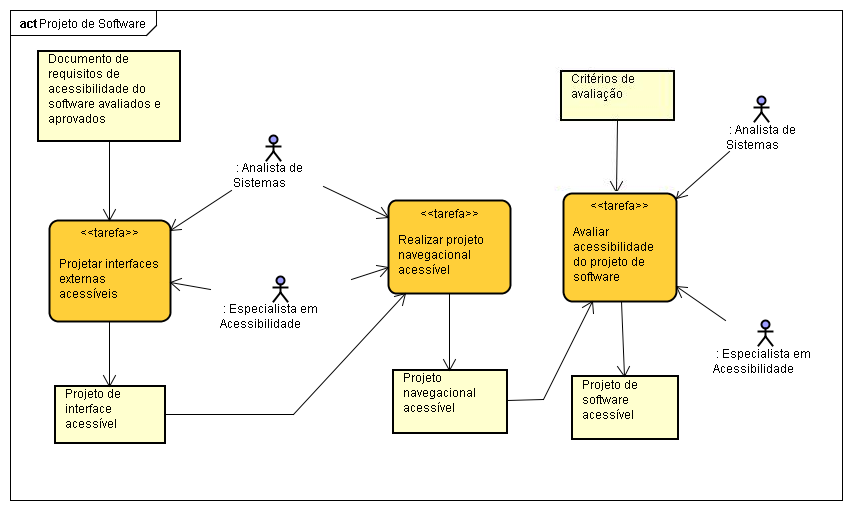
\includegraphics[width=.8\textwidth,height=200px]{./images/subprocesso5.png}
\caption{Tarefas para o subprocesso de projeto de software \citep{maia:10}}
\label{fig:sub5}
\end{figure}

As tr�s tarefas deste subprocesso s�o de extrema import�ncia, e impactam
diretamente na acessibilidade do produto final. O artefato XML/XMI gerado no
subprocesso anterior passar� por cada tarefa deste subprocesso, de forma que,
al�m da sa�da da tarefa \textbf{Avaliar a acessibilidade do projeto de software}
e gerar o artefato \textbf{Projeto de software acess�vel}, esta tarefa tamb�m
gerar� um artefato de projeto de software no formato XML/XMI, com elementos de
acessibilidade embutidos.

A proposta deste trabalho enseja que as subtarefas das tarefas pertencentes a
esse subprocesso j� comecem a contar com crit�rios de sucesso do documento de
diretrizes de acessibilidade escolhido.
Desta forma, torna-se mais f�cil relacionar os pontos cr�ticos de acessibilidade do
projeto de interface e navega��o nos passos posteriores, principalmente porque
um software automatizado n�o consegue fazer algumas verifica��es levando em
considera��o o contexto sem�ntico (por exemplo, ordem de navega��o), e esses
pontos cr�ticos devem ser revisados posteriormente.

Al�m disso, � necess�rio esclarecer que o padr�o de conformidade para o projeto
� definido na tarefa 1.1 do subprocesso 1 (Elicita��o dos Requisitos do
Sistema). Os padr�es e ferramentas dispon�veis levam em considera��o o
reconhecido padr�o WCAG 2.0. Contudo, a necessidade de conformidade com
outros padr�es de acessibilidade leva a necessidade de um
monitoramento constante por parte do especialista em acessibilidade, pois nem sempre as
t�cnicas para a implementa��o do que � cobrado no padr�o est�o dispon�veis (por
exemplo, � poss�vel que um \textit{software} precise estar em conformidade com o
modelo \textit{Section 508}, mas esse padr�o n�o explicita o que deve ser
feito para que o n�vel de acessibilidade pretendido seja alcan�ado).

O especialista em acessibilidade deve associar os elementos de interface e
navega��o, utilizando da ferramenta \gls{case} aos requisitos
provenientes da etapa anterior. Al�m disso � poss�vel mapear, se aplic�vel, t�cnicas de implementa��o
de acessibilidade.

Um projeto �til para essa finalidade � \textit{AEGIS Ontology}
\footnote{http://www.aegis-project.eu/index.php?option=com\_content\&view=article\&id=107\&Itemid=65},
que define ontologias de acessibilidade na \textit{Web}. O principal objetivo do
projeto � mapear os conceitos de acessibilidade, e como eles podem ser mapeados
dentro de um cen�rio de acessibilidade.

O projeto � apoiado pelo \textit{Accessible Consortium}
\footnote{http://www.accessible-eu.org/index.php/consortium.html}, que
disponibiliza uma p�gina para a consulta das novidades da iniciativa
\footnote{http://www.accessible-eu.org/index.php/ontology.html}. A vers�o atual
� a 5.1

As ontologias s�o descritas no formato \gls{owl}, padr�o definido pela \gls{w3c}
em 2004\footnote{http://www.w3.org/TR/owl-features/}, que est� na vers�o 1.0
mas j� possui uma vers�o candidata � 2.0, lan�ada em 2012
\footnote{http://www.w3.org/TR/owl2-overview/}. As ontologias descritas est�o no padr�o 1.0.

O projeto vai al�m de realizar o mapeamento dos conceitos de acessibilidade e
cen�rios. Os arquivos disponibilizados mapeam o modelo WCAG 2.0 (incluindo
t�cnicas de implementa��o, crit�rios de sucesso e falha, etc), leitores de tela,
navegadores textuais, lentes de aumento, WAI/ARIA, entre outros. � poss�vel
navegar pelas ontologias via navegador
\footnote{http://160.40.50.89/Accessible\_Ontology/Version5.1/AccessibleOntologyOWLDoc/index.html},
ou explorar os arquivos confortavelmente atrav�s do software \textit{Proteg�}
\citep{Noy01creatingsemantic}.

No estudo de caso, ser� utilizado as ontologias definidas por este projeto, onde
ser� explicado com mais detalhes como elas ser�o utilizadas.

Ao final deste subprocesso, a ferramenta \gls{case} j� deve ter as associa��es dos requisitos de acessibilidade com os
itens de interface e navega��o (j� incluindo a associa��o com o WCAG 2.0), bem como os outros artefatos modelados 
no subprocesso anterior. A matriz de rastreabilidade pode ser gerada novamente,
dessa vez mais completa, pois mais dados est�o dispon�veis neste ponto do
processo.

\section{Subprocesso 6 - Constru��o do Software}

 O objetivo do subprocesso 6 � produzir unidades de software execut�veis que
 apropriadamente refletem o projeto de software \citep{maia:10}.
 
 O MTA insere quatro tarefas de acessibilidade, conforme mostrado na Figura
\ref{fig:sub6}.

\begin{figure}[ht]
\centering
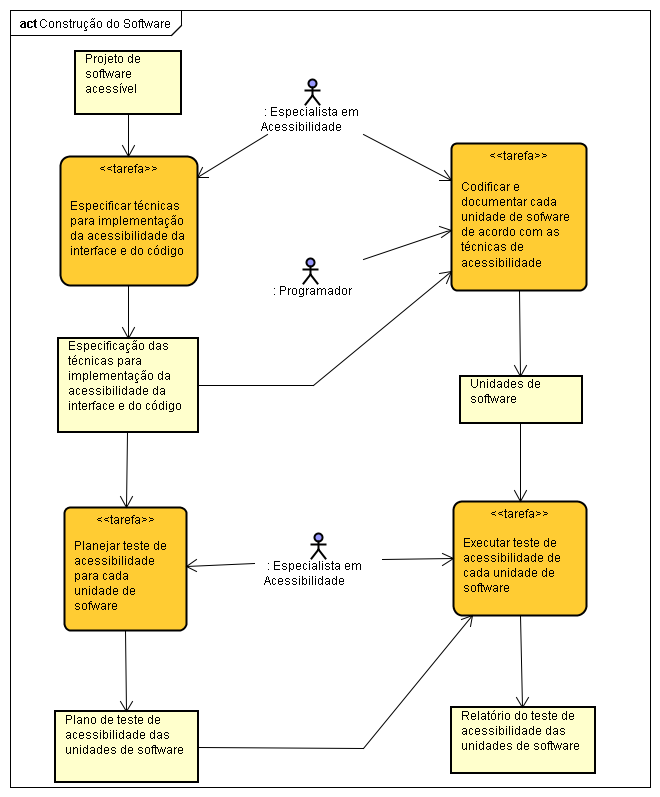
\includegraphics[width=.8\textwidth,height=350px]{./images/subprocesso6.png}
\caption{Tarefas para o subprocesso de constru��o do software \citep{maia:10}}
\label{fig:sub6}
\end{figure}

A tarefa 6.1 (Especificar T�cnicas para Implementa��o da Acessibilidade da
Interface e do C�digo) visa explicitar as t�cnicas de implementa��o de
acessibilidade, refletidas no projeto de software. Como dito anteriormente, o
padr�o de conformidade j� deve ter sido escolhido no subprocesso 1. Apesar dos padr�es
de acessibilidade serem diferentes em ess�ncia, existe uma grande intersec��o no que se
refere as t�cnicas utilizadas para implementa��o efetiva da acessibilidade no produto.
As regras para implementa��o do padr�o e-Mag 3.0 s�o muito parecidas com as do padr�o WCAG 2.0,
e a tend�ncia � que haja uma homogeneiza��o dos esfor�os em desenvolver produtos acess�veis, principalmente
como a evolu��o do \gls{html} 5. 

Os modelos WCAG 2.0 e e-Mag 3.0 j� possuem t�cnicas de acessibilidade presentes
em seus respectivos documentos. Esse � o momento de relacionar as
especificidades do projeto de software com as t�cnicas de acessibilidade do modelo escolhido. Caso nenhum
modelo conhecido ou algum modelo n�o usual tenha sido escolhido, as t�cnicas de
implementa��o de acessibilidade dever�o ser explicitamente relacionadas no
projeto, e, para isso, � fundamental o aux�lio de um especialista em
acessibilidade.

Por conveni�ncia, as t�cnicas utilizadas ser�o as do WCAG 2.0, pelo fato de j� estarem mapeadas nos arquivos
\gls{owl} descritos anteriormente.

Devido ao escopo do trabalho, apesar serem extremamente importantes, as tarefas
\textbf{Planejar teste de acessibilidade para cada unidade de software} e
\textbf{Executar teste de acessibilidade de cada unidade de software} n�o foram
consideradas.

A tarefa 6.2 (Codificar e documentar cada unidade de software de acordo com as
t�cnicas de acessibilidade) recebe benef�cios diretos dos passos anteriores,
pois o projeto j� cont�m os pontos cr�ticos de acessibilidade explicitados. 
Ferramentas \gls{case}, neste ponto, comumente geram c�digo
(\textit{stub}), utilizando artefatos como diagramas de classe, de sequ�ncia e casos de uso. O c�digo
gerado j� poderia conter tra�os de documenta��o associados aos requisitos de acessibilidade.
Uma maneira imediata de documentar c�digo � adicionando coment�rios padronizados, de forma que os requisitos
de acessibilidade possam ser localizados. Dependendo da linguagem de programa��o
utilizada, podem ser utilizadas anota��es para referenciar os modelos (a
linguagem \textit{Java} permite o uso de anota��es).

Para incorporar a rastreabilidade
dos requisitos no c�digo gerado pelas ferramentas em forma de coment�rio de c�digo, temos as seguintes abordagens:

\begin{enumerate}
  \item A ferramenta de modelagem gera os c�digos, e a partir destes, a ferramenta \gls{case} proposta incluiria os coment�rios
  de rastreabilidade;
  \item A ferramenta \gls{case} proposta substituiria o gerador de c�digo, realizando todo o trabalho e gerando o c�digo j� documentado.
  \item O gerador de c�digo � customizado para que gere o c�digo e os
  coment�rios de associa��o.
\end{enumerate}

\textbf{EXPLICAR A ABORDAGEM ESCOLHIDA E O MOTIVO}

\section{Escolha das Ferramentas e Tecnologias}

A proposta deste trabalho � demonstrar a rastreabilidade dos requisitos de
acessibilidade no processo de desenvolvimento de \textit{software},
independente de ferramenta ou tecnologia adotada pelos analistas e
desenvolvedores.

J� existem iniciativas, principalmente corporativas, que permitem agregar os
requisitos levantados aos artefatos do processo de desenvolvimento.
\citet{hovater:08} mostra como construir relat�rios de rastreabilidade usando os
programas \textit{IBM Rational Software Architect}\footnote{http://www-142.ibm.com/software/products/br/pt/ratisoftarch/},
\textit{IBM Rational RequisitePro}\footnote{http://www-142.ibm.com/software/products/br/pt/reqpro/} e \gls{birt}
para \textit{WebSphere}\footnote{http://www-01.ibm.com/software/websphere/}.

O software \textit{Enterprise Architect} da empresa \textit{Sparx Systems}\footnote{http://www.sparxsystems.com/enterprise\_architect\_user\_guide/index.html}
permite utilizar diagramas de requisitos\footnote{http://www.sparxsystems.com/enterprise\_architect\_user\_guide/modeling\_languages/requirements\_diagram.html},
que s�o extens�es dos diagramas tradicionais da \gls{uml}, permitindo a
rastreabilidade do
modelo\footnote{http://www.sparxsystems.com/enterprise\_architect\_user\_guide/navigate\_search\_and\_trace/traceability.html}.
Contudo, n�o foi encontrado na literatura trabalhos que tratem especificamente da rastreabilidade dos requisitos de acessibilidade dentro do processo de um
desenvolvimento de \textit{software}.

Dessa forma, para demonstrar a proposta deste trabalho, ser� constru�da uma
ferramenta \gls{case}, nos moldes descritos na se��o \ref{linktocase}. A seguir
� elencado os principais elementos usados para a demostra��o deste trabalho.

\begin{itemize}
  \item \gls{mta} - Processo de Desenvolvimento de \textit{Software} com tarefas
  de acessibilidade
  \item \textit{Eclipse Juno} - \gls{ide}
  \item \textit{Requirement Designer v0.8.0}\footnote{http://marketplace.eclipse.org/node/407399\#.UR43GaXC1VJ} - 
  \textit{plugin} de gerenciamento de
  requisitos
  \item \textit{UML Designer v2.1.0}\footnote{http://marketplace.eclipse.org/content/uml-designer-indigo-version\#.UR43OaXC1VI} - 
  \textit{plugin} de modelagem \gls{uml}
  \item \textit{UML to Java Generator v1.0.2}\footnote{http://marketplace.eclipse.org/content/uml-java-generator\#.UR44XKXC1VI} - 
  \textit{plugin} de gera��o de c�digo 
  \item \textit{Java JRE7 e JDK1.7}\footnote{http://www.oracle.com/technetwork/java/index.html} 
  - Linguagem para desenvolvimento de \textit{plugins} e c�digo final do produto
  \item Ontologias para implementa��o das diretrizes do \gls{wcag} 2.0.
\end{itemize}

O \textit{Eclipse} � uma plataforma madura e foi escolhido como \gls{ide} por
v�rios motivos. Ele serve como base para para diversos produtos e tecnologias baseadas em uma \gls{ide},
provendo uma \gls{api} para facilitar a integra��o \citep{5386785}.
O desenvolvimento de \textit{plugins} para o \textit{Eclipse} � feito diretamente na \gls{ide}, de forma pr�tica e 
transparente\footnote{Um tutorial de desenvolvimento de plugins para o Eclipse
pode ser encontrado em http://www.ibm.com/developerworks/br/library/os-ecplug/}, tendo ampla documenta��o a respeito. 
A linguagem utilizada para o desenvolvimento do \textit{plugin} � linguagem \textit{Java}, assim como o c�digo gerado 
pelo \textit{plugin} de exporta��o.

O pacote de modelagem inicialmente instalado foram os \textit{plugins} \gls{emf} propostos pelo \textit{Eclipse}, notadamente
o \textit{Ecore Tools}\footnote{http://www.eclipse.org/modeling/emft/?project=ecoretools}, parte integrante do \gls{emft}. Contudo,
os diagramas fornecidos por \textit{default} n�o satisfizeram aos anseios de modelagem, pois n�o contemplavam diagramas de sequ�ncia ou de 
casos de uso, por exemplo. Por esse motivo, o \textit{plugin} escolhido foi o \textit{UML Designer}, que utiliza como base o pacote \gls{emf} (portanto gera modelos \gls{emf}), 
mas extende os modelos existentes para que se adequem aos modelos \gls{uml} na sua vers�o 2.4. 

O \textit{plugin} inicialmente escolhido para o gerenciamento de requisitos foi o \textit{ProR}\footnote{http://www.eclipse.org/rmf/pror/},
que por sua vez � parte do projeto \gls{rmf} e \gls{emf} do \textit{Eclipse}. O objetivo do projeto \gls{rmf} � implementar o 
padr�o \textit{OMG ReqIF}\footnote{http://www.omg.org/spec/ReqIF/}
em forma de modelos \gls{emf}. Contudo, o \gls{rmf} se encontra atualmente na 0.6.0, e o \textit{plugin} n�o fornecia a 
funcionalidade de liga��o entre os modelos e os requisitos. Assim, modos alternativos de relacionamento entre os modelos e os requisitos
deveriam ser implementados, tornando invi�vel o desenvolvimento do trabalho. Portanto, o \textit{plugin} escolhido para o gerenciamento
de requisitos foi o \textit{Requirement Designer}, que permite realizar a associa��o dos requisitos com qualquer modelo \gls{emf}.

Os \textit{plugins} de modelagem e gerenciamento de requisitos s�o desenvolvidos pela \textit{Obeo}\footnote{http://www.eclipse.org/membership/showMember.php?member\_id=863},
portanto, para permitir uma integra��o suave entre as ferramentas, o \textit{plugin} escolhido para gera��o de c�digo foi o 
\textit{UML to Java Generator}, desenvolvido pela mesma empresa. Os \textit{plugins} s�o disponibilizados sob a licen�a \textit{Eclipse Public License v
1.0}\footnote{http://www.eclipse.org/legal/epl-v10.html}, assim como a pr�pria \gls{ide}. Dessa forma, � poss�vel
estudar, alterar e customizar seus componentes para atingir aos objetivos do trabalho.

A Figura \ref{fig:association} mostra o comportamento e relacionamento das
ferramentas, tecnologias e atores envolvidos no desenvolvimento do produto, que
deve ser interpretada da seguinte forma:

\begin{itemize}
  \item O \gls{mta} � o processo de desenvolvimento, e deve permear todas as
  fases do processo;
  \item O especialista em acessibilidade (\textit{Accessibility Expert}) deve
  participar das fases de desenvolvimento especificadas no \gls{mta};
  \item Os requisitos devem ser coletados e informados na fase de engenharia de
  requisitos (utilizando a ferramenta \textit{Requirement
  Designer}), e os modelos e artefatos \gls{uml} devem ser gerados (utilizando a
  ferramenta \textit{UML Designer}) O especialista em acessibilidade deve
  auxiliar a alimenta��o destes dados, filtrando os requisitos de acessibilidade para que eles sejam
  associados aos modelos \gls{uml} (utilizando a ferramenta
  \textit{Requirement Designer});
  \item A ferramenta proposta recupera as associa��es dos requisitos e modelos
  \gls{uml} (apenas aos que dizem respeito � acessibilidade), permitindo que o
  especialista especifique as t�cnicas de implementa��es de acessibilidade para
  cada uma das associa��es. As t�cnicas, diretrizes, abordagens e o que mais
  dizer respeito a implementa��o t�cnica da associa��o est�o armazenadas em
  arquivos \gls{owl} embutidos na ferramenta;
  \item A ferramenta de gera��o de c�digo produzir� o c�digo \textit{stub} a
  partir dos modelos \gls{uml}, adicionando as refer�ncias �s associa��es de
  acessibilidade quando necess�rio;
  \item O(s) desenvolvedor(res) refinam o c�digo at� que o mesmo esteja apto a
  se tornar o produto acess�vel que ser� entregue.
\end{itemize}

\begin{figure}[ht]
\centering
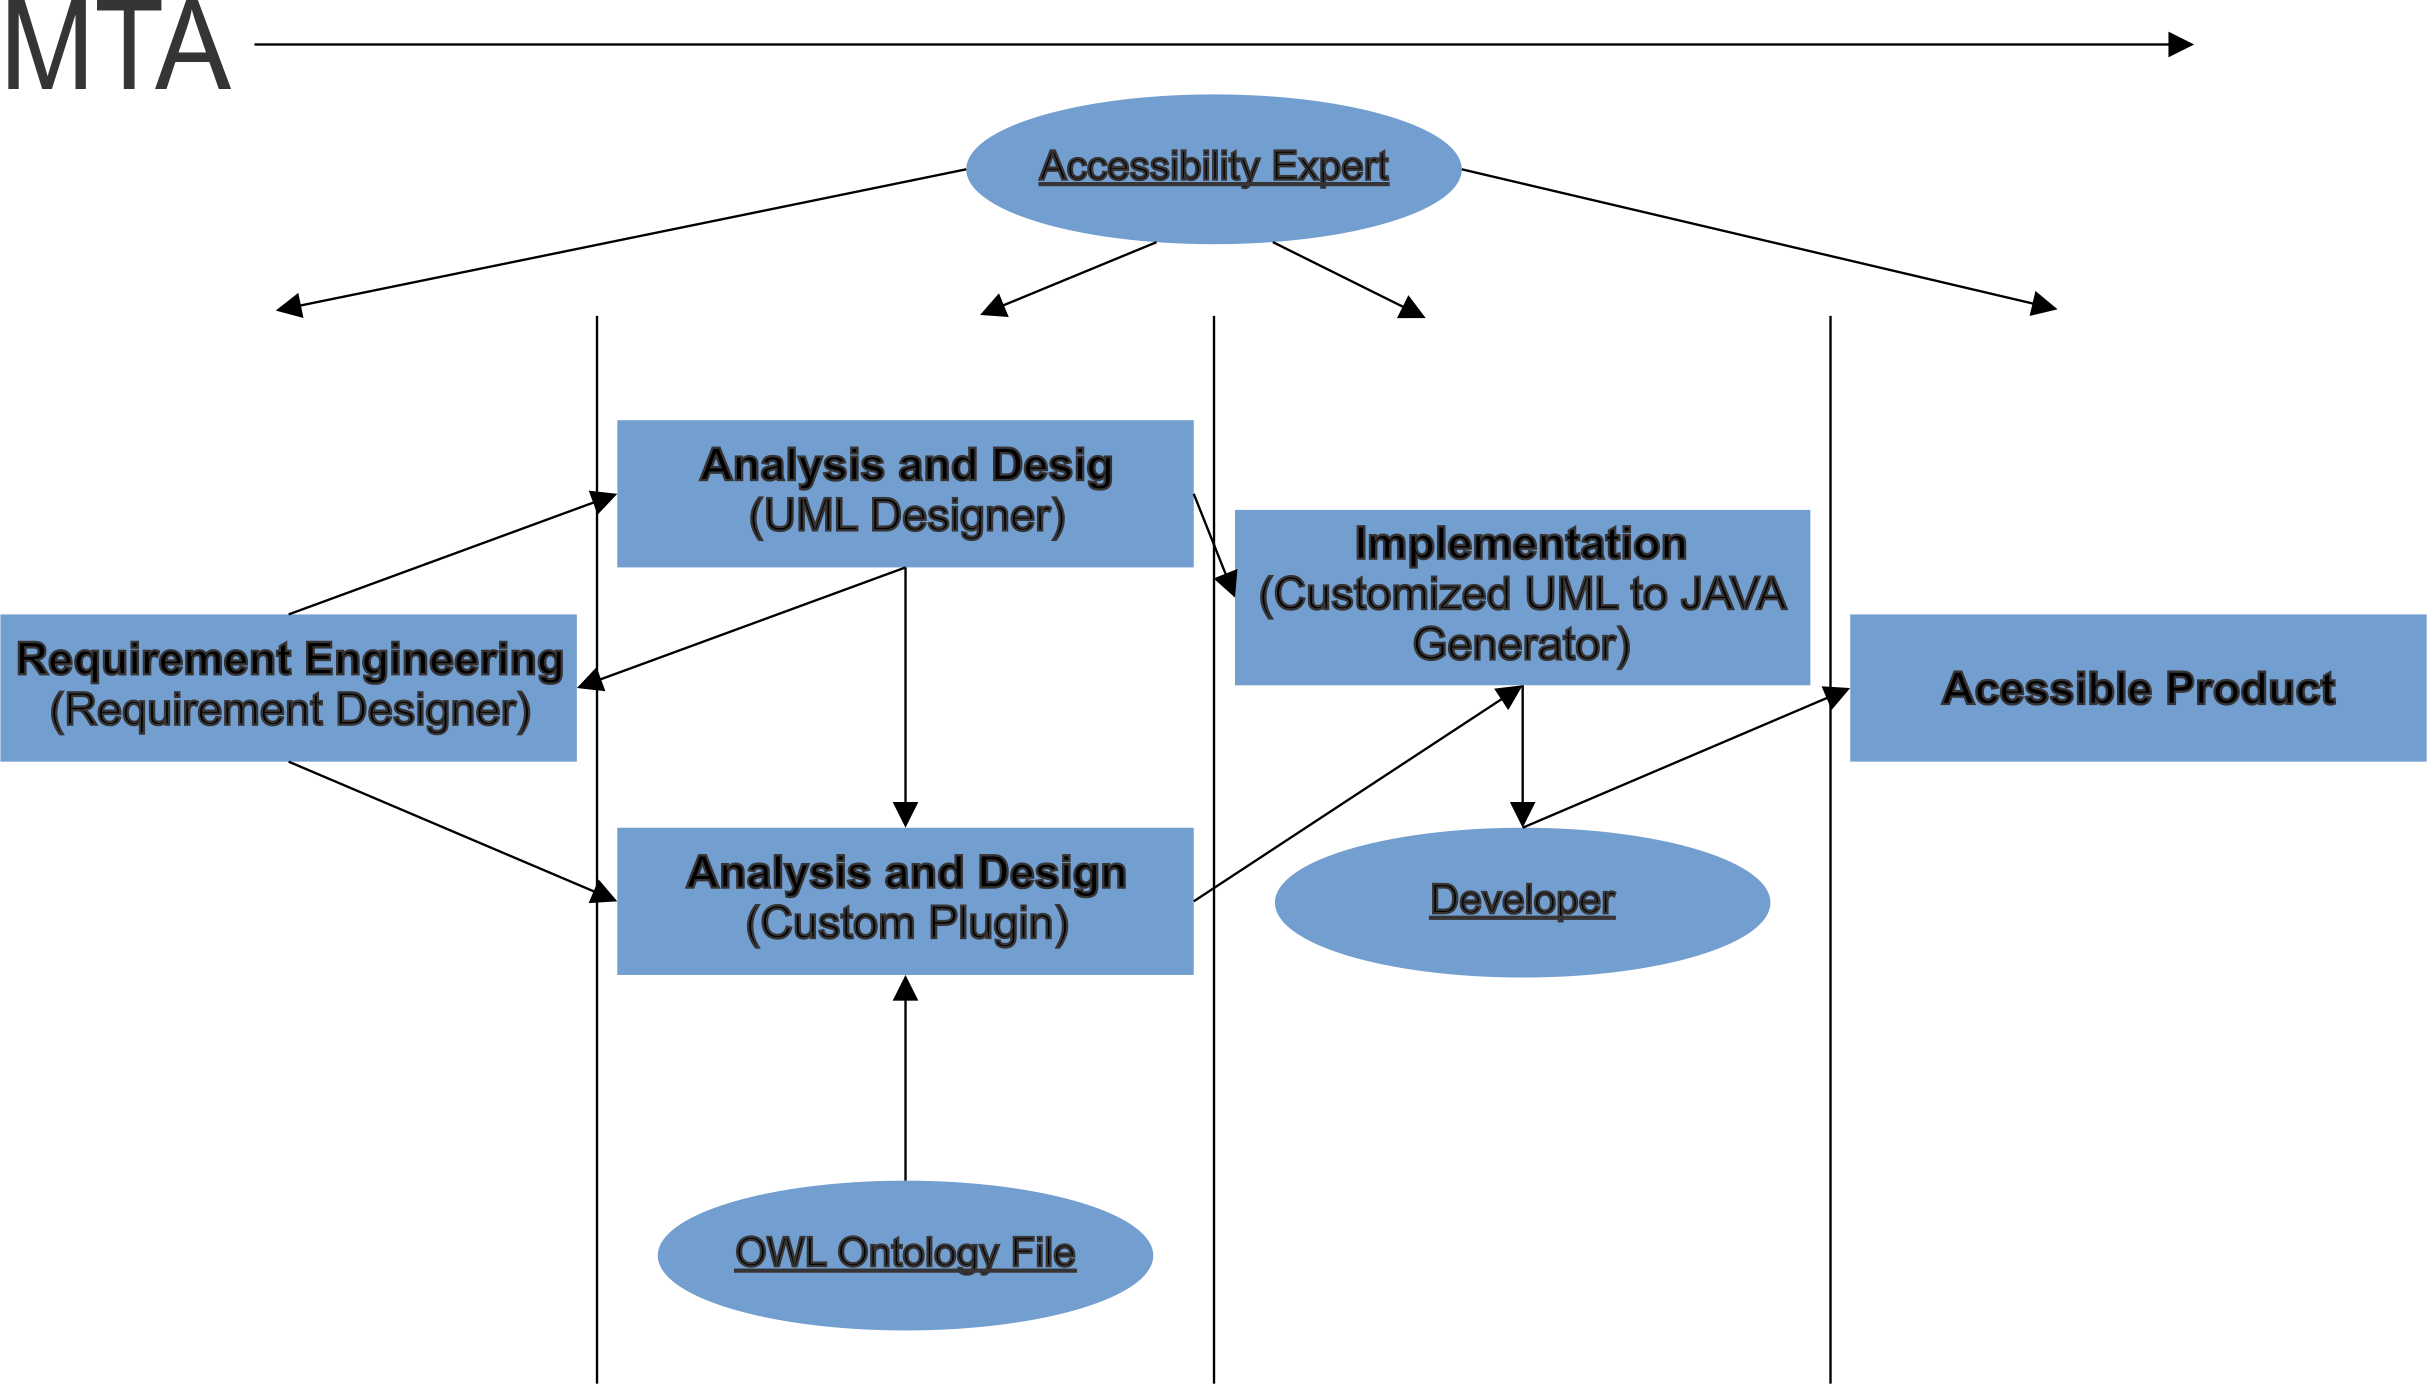
\includegraphics[width=.8\textwidth]{./images/developmentNew.png}
\caption{Associa��o das ferramentas e atores no contexto to trabalho}
\label{fig:association}
\end{figure}

\section{Constru��o da Ferramenta}

O \textit{plugin} constru�do utiliza quatro elementos externos que precisam ser
detalhados:

\begin{itemize}
  \item O reposit�rio dos requisitos
  \item O requisito
  \item O modelo \gls{uml}
  \item A t�cnica de acessibilidade, representado pela ontologia
\end{itemize}

A Figura \ref{fig:reqdesignerexample} mostra a execu��o da ferramenta
\textit{Requirement Designer} e o cadastro de algumas categorias e requisitos
como exemplo.

\begin{figure}[ht]
\centering
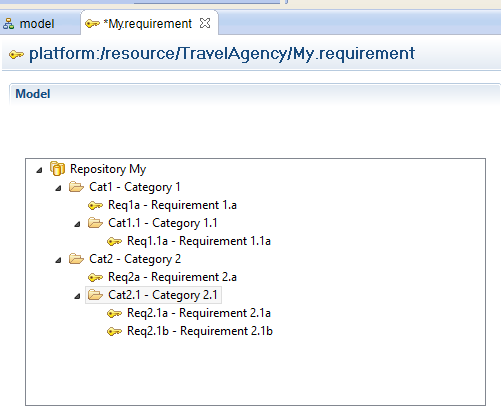
\includegraphics[width=.8\textwidth]{./images/requirementDesignerExample.png}
\caption{Execu��o da ferramenta \textit{Requirement Designer}}
\label{fig:reqdesignerexample}
\end{figure}

O diagrama de classes visualizado na Figura \ref{fig:reqdesigner_classdiagram}
demonstra o n�cleo de funcionamento do \textit{plugin Requirement Designer},
que possui os dois primeiros elementos listados anteriormente.
Existe um reposit�rio (\textit{Repository}), que pode conter zero ou mais
categorias principais (\textit{Category}). Cada categoria principal pode conter
0 ou mais requisitos (\textit{Requirement}), e tamb�m pode conter 0 ou mais
subcategorias (\textit{Category}), recursivamente. Os requisitos podem ser do
tipo funcionais ou n�o-funcionais (neste \textit{plugin} tratados como
requisitos t�cnicos).

\begin{figure}[ht]
\centering
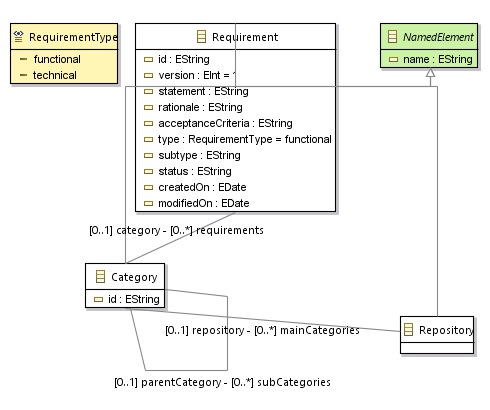
\includegraphics[width=.8\textwidth]{./images/requirement_package_entities.png}
\caption{Diagrama de classes do \textit{plugin} Requirement Designer}
\label{fig:reqdesigner_classdiagram}
\end{figure}

O diagrama de classes foi gerado usando o \gls{emf} (especificamente a
ferramentas \textit{Ecore Model}), resultando nas classes java representativas
do modelo (usando a ferramenta de transforma��o \textit{Ecore Generator Model}).
Na pr�tica, significa dizer que, uma vez tendo o diagrama de classes no modelo
\textit{Ecore}, seja poss�vel utilizar as classes java resultantes e,
principalmente, que o arquivo de sa�da da ferramenta \textit{Requirement
Designer} possa ser lido e interpretado de forma simplificada como os objetos
corretos do \textit{plugin}.

A ferramenta para gerar os artefatos \gls{uml} � a \textit{UML Designer}. A
ferramenta usa a \gls{api} do \textit{Eclipse (org.eclipse.uml2.uml)}, que por
sua vez � persistida usando \gls{emf}. Por esse motivo, a ferramenta de
gerenciamento de requisitos consegue gerar uma associa��o entre os requisitos e
qualquer elemento presente na \gls{api}.

A Figura \ref{fig:usecaseexample} mostra um diagrama de casos de uso de exemplo
gerado pela ferramenta \textit{UML Designer}.

\begin{figure}[ht]
\centering
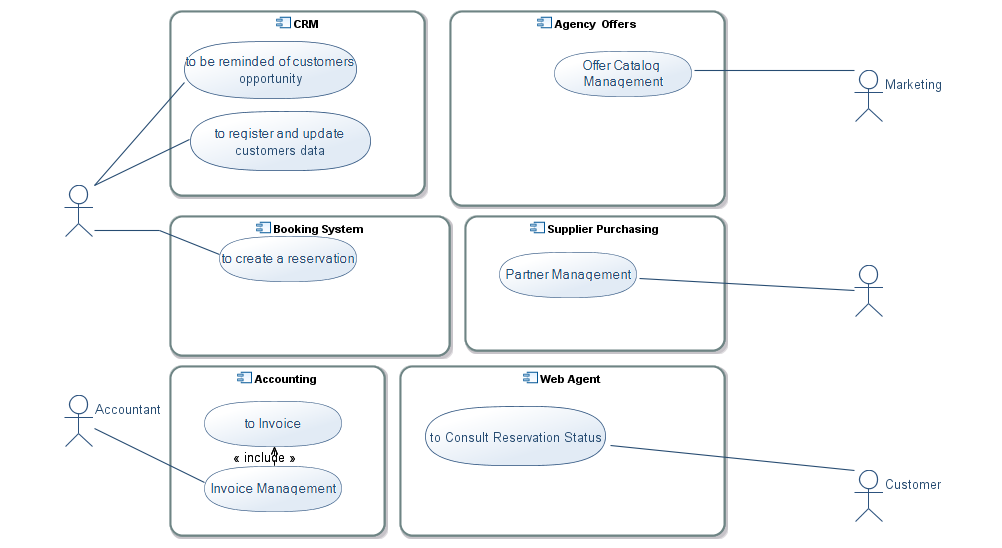
\includegraphics[width=.8\textwidth]{./images/usecaseexample.png}
\caption{Exemplo de um diagrama de casos de uso gerado pela ferramenta
\textit{UML Designer}}
\label{fig:usecaseexample}
\end{figure}

A ferramenta \textit{Requirement Designer} utiliza refer�ncias \gls{emf}
(elementos \textit{proxy}) para associar os modelos \gls{uml} gerados pela
ferramenta \textit{UML Designer}, significando que os objetos referenciados n�o
s�o escritos no arquivo \gls{xml} de destino. Assim, o modelo pode ser alterado,
e o objeto sempre estar� atualizado no arquivo referenciado. Essa mesma t�cnica
ser� usada no modelo de dados a ser constru�do pela ferramenta proposta, com
exce��o dos objetos referentes �s ontologias de acessibilidade.

As ontologias de acessibilidade s�o descritas no padr�o \gls{owl}, que tem por
base o formato \gls{rdf}. Para efetuar a leitura dos arquivos \gls{owl},
utilizamos a \textit{OWL API}, que por sua vez � utilizado pelo
\textit{software Prot�g�}, \textit{software} este muito �til para visualizar de
forma gr�fica os elementos e relacionamentos descritos nas ontologias. Este
\textit{software} foi usado diversas vezes para descobrir quais os elementos da
ontologia e como eles deveriam ser acessados atrav�s da api. A figura
\ref{fig:protege} mostra um dos arquivos de ontologias usados no trabalho aberto
para consulta.

\begin{figure}[ht]
\centering
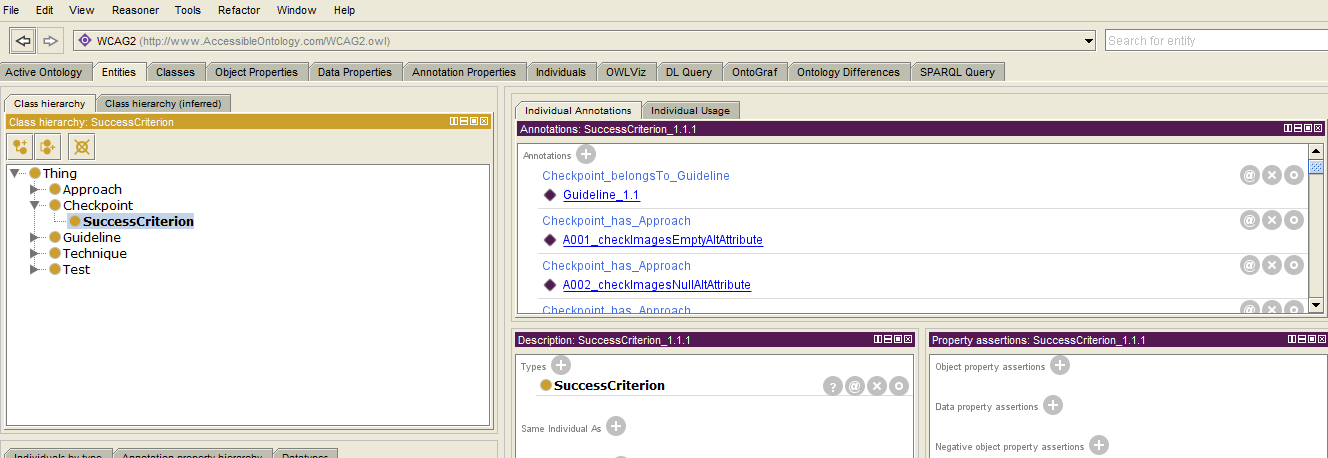
\includegraphics[width=.8\textwidth]{./images/protege.png}
\caption{Exemplo do arquivo WCAG2.owl aberto no \textit{software Prot�g�}}
\label{fig:protege}
\end{figure}

Diante do exposto, � poss�vel apresentar o diagrama de classes da ferramenta
proposta, aqui denominada como \textit{AccTrace}, vis�vel na Figura
\ref{fig:acctraceclassdiagram}.

\begin{figure}[ht]
\centering
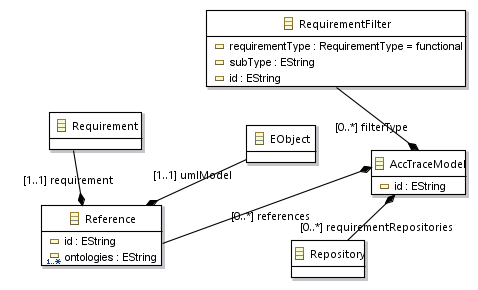
\includegraphics[width=.8\textwidth]{./images/acctraceclassdiagram.png}
\caption{Diagrama de classes da ferramenta proposta (\textit{AccTrace})}
\label{fig:acctraceclassdiagram}
\end{figure}

O diagrama de classes deve ser interpretado da seguinte forma: A classe
principal � a \textit{AccTraceModel}, que armazena as refer�ncias para os
reposit�rios dos requisitos (\textit{Repository}), e tamb�m objetos de
refer�ncia �s associa��es dos requisitos, modelos e t�cnicas
de implementa��o de acessibilidade (\textit{Reference}). Esse objeto referencia
um requisito (\textit{Requirement}), um diagrama \gls{uml} (\textit{EObject}) e
1 ou mais t�cnicas de implementa��o de acessibilidade, representadas aqui pela
sele��o das ontologias dispon�veis. As refer�ncias �s ontologias s�o persistidas
atrav�s de suas \gls{iri} (uma generaliza��o de \gls{uri}) em forma de \textit{String}.
Al�m disso, devido ao grande n�mero de requisitos poss�veis no projeto e
considerando o fato de que apenas os requisitos de acessibilidade sejam
importantes para a associa��o � t�cnicas de implementa��o de acessibilidade, � previsto no modelo tamb�m a inclus�o de filtros dos requisitos (\textit{RequirementFilter}), para n�o poluir a
visualiza��o dos requisitos na ferramenta.

A ferramenta possui tr�s vis�es principais, de acordo com a Figura
\ref{fig:acctrace}: o editor (\textit{AccTrace Editor}), onde � poss�vel alterar
os reposit�rios dos requisitos e gerar as associa��es entre os modelos
\gls{uml}, requisitos e t�cnicas de implementa��o; a vis�o dos requisitos
(\textit{Requirement Associations}), onde � poss�vel visualizar quais os
requisitos associados ao modelo \gls{uml} selecionado no editor; e a vis�o das
t�cnicas j� implementadas (\textit{Accessibility Specifications View}), onde �
poss�vel visualizar as t�cnicas de implementa��o j� associadas, de acordo com o
modelo \gls{uml} selecionado no editor e o requisito de acessibilidade
selecionado na vis�o dos requisitos, bem como remover as t�cnicas de
implementa��o associadas. As tr�s vis�es s�o importantes para o correto
funcionamento da ferramenta.

\begin{figure}[ht]
\centering
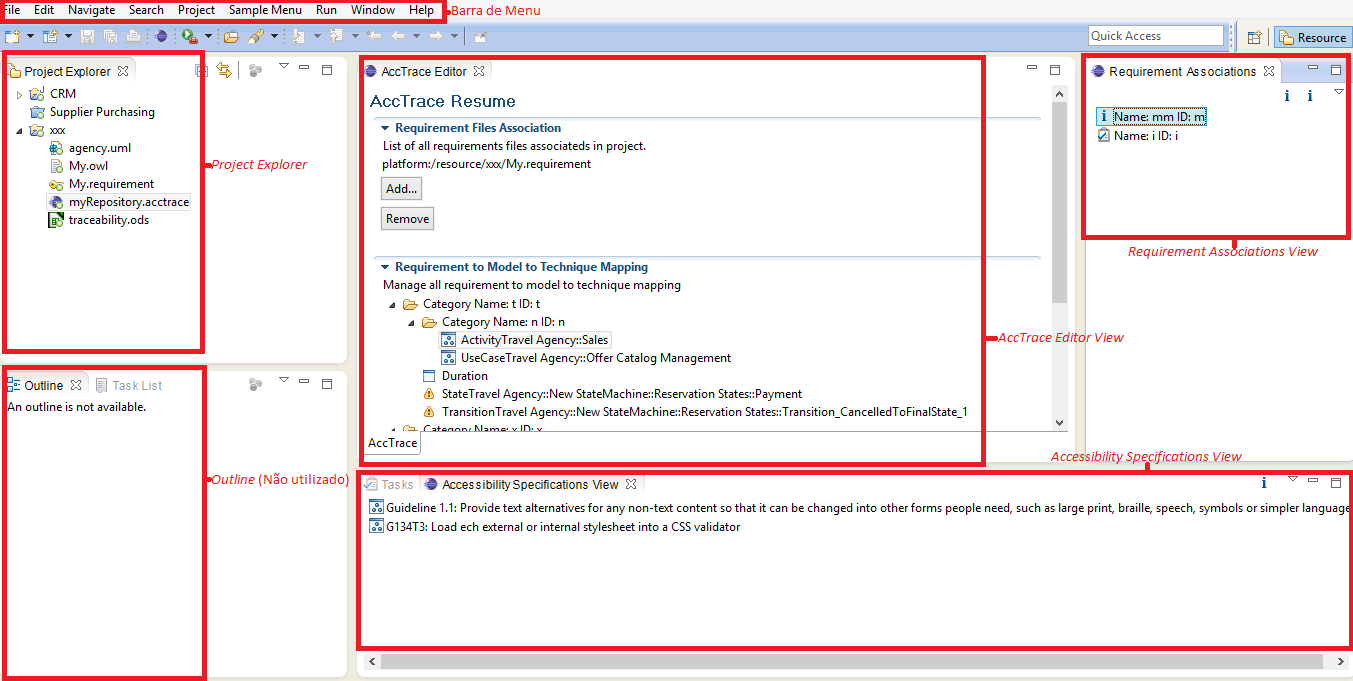
\includegraphics[width=.8\textwidth]{./images/acctrace.png}
\caption{Visualiza��o da ferramenta \textit{AccTrace} na tela principal do
\textit{Eclipse}}
\label{fig:acctrace}
\end{figure}

Uma vez selecionado o modelo \gls{uml} e o requisito, � poss�vel efetuar a
associa��o da t�cnica de implementa��o de acessibilidade, clicando com o bot�o
direito do mouse em cima do modelo \gls{uml}, conforme demonstrado na Figura
\label{fig:rightclick}.

\begin{figure}[ht]
\centering
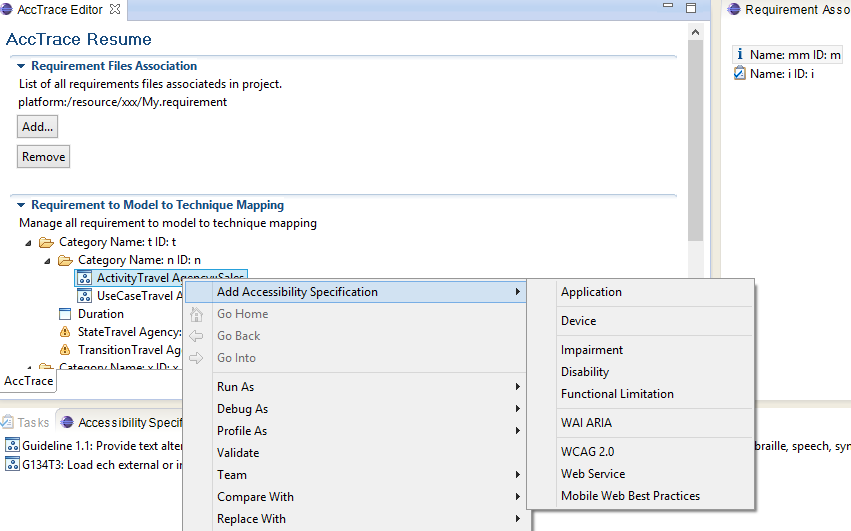
\includegraphics[width=.8\textwidth]{./images/rightclick.png}
\caption{Procedimento para efetuar a associa��o da t�cnica de implementa��o de
acessibilidade}
\label{fig:rightclick}
\end{figure}

O menu mostrado na Figura foi projetado levando em conta
a an�lise e estudo das ontologias dispon�veis, efetuados na ferramenta
\textit{Prot�g�}. � poss�vel entender o relacionamento dos elementos e
ontologias observando a Figura \ref{fig:ontologyrelationship}.

\begin{figure}[ht]
\centering
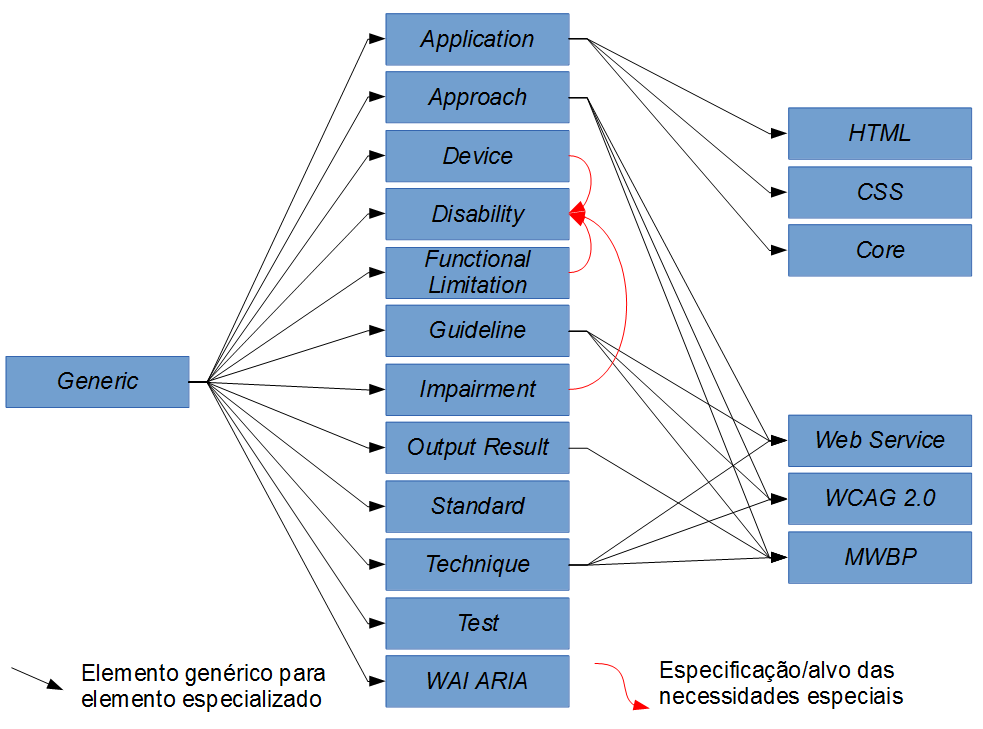
\includegraphics[width=.8\textwidth]{./images/ontologyrelationship.png}
\caption{Relacionamento entre as ontologias}
\label{fig:ontologyrelationship}
\end{figure}

Para este trabalho, uma das ontologias mais importantes � a ontologia denominada
\textit{WCAG 2.0}, pois � esta ontologia que comporta as t�cnicas de
implementa��o de acessibilidade que efetivamente ser�o utilizadas. As outras
ontologias, apesar de acess�rias, podem ser utilizadas para refor�ar as t�cnicas
j� referenciadas. 

A ontologia \textit{WCAG 2.0} possui 5 grupos a serem escolhidos, conforme
mostra a Figura \ref{fig:wcag2groups}: abordagens, testes, crit�rios de
sucesso, diretrizes ou t�cnicas. Cada um desses grupos cont�m os elementos que
efetivamente devem ser selecionados para que a associa��o seja conclu�da.
Tomando como base a escolha do subgrupo crit�rios de sucesso, podemos ver as
op��es dispon�veis mostradas na Figura \ref{fig:successcriterion}. Os elementos
internos das ontologias s�o diferentes, dependendo qual seu tipo e objetivo. A
Figura \ref{fig:successcriterion127} mostra quais os elementos da ontologia
escolhida como exemplo (\textit{WCAG2 SuccessCriterion 1.2.7}):
ela possui uma descri��o, uma prioridade, um ID e um nome, al�m de
relacionamentos com outras ontologias que aqui foram omitidas. Uma vez
selecionada a ontologia apropriada, um clique no bot�o OK faz com que a
associa��o seja persistida ao modelo.

\begin{figure}[ht]
\centering
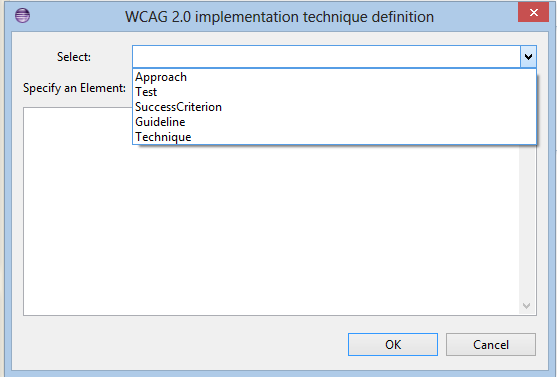
\includegraphics[width=.8\textwidth]{./images/wcag2groups.png}
\caption{Grupos a serem selecionados a partir da ontologia \textit{WCAG 2.0}}
\label{fig:wcag2groups}
\end{figure}

\begin{figure}[ht]
\centering
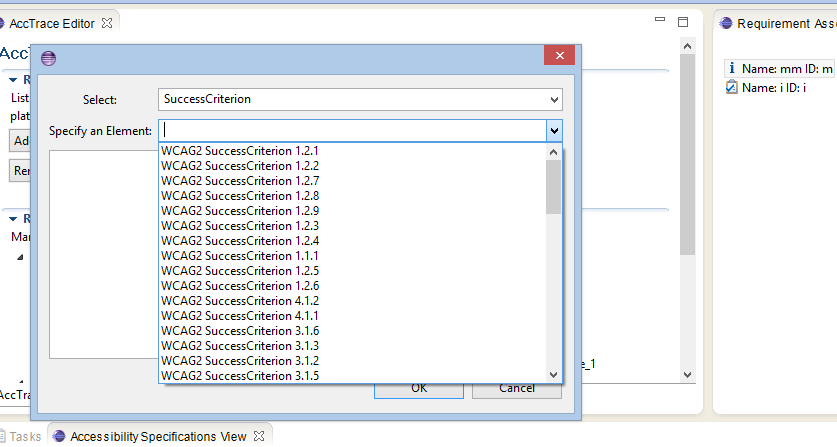
\includegraphics[width=.8\textwidth]{./images/successcriterion.png}
\caption{Elementos dispon�veis para a ontologia \textit{SuccessCriterion}}
\label{fig:successcriterion}
\end{figure}

\begin{figure}[ht]
\centering
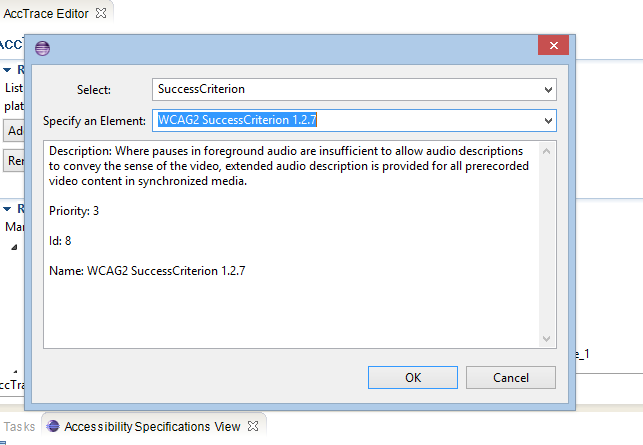
\includegraphics[width=.8\textwidth]{./images/successcriterion127.png}
\caption{Sele��o da ontologia \textit{WCAG2 SuccessCriterion 1.2.7}}
\label{fig:successcriterion127}
\end{figure}

� poss�vel rastrear os requisitos, modelos \gls{uml} e t�cnicas de implementa��o
atrav�s da gera��o de uma matriz de rastreabilidade. Neste trabalho foi
utilizado o \textit{Apache ODF
Toolkit}\footnote{http://incubator.apache.org/odftoolkit/} para gera��o do
documento de rastreamento com formato \gls{ods}, atrav�s da \gls{api} de alto
n�vel
\textit{Simple}\footnote{http://incubator.apache.org/odftoolkit/simple/index.html}.
No documento, s�o geradas tr�s planilhas: Requerimentos x Modelos, Requerimentos
x T�cnicas e Modelos x T�cnicas. A planilha Requerimentos x Modelos lista uma
matriz de todos os requerimentos associados aos respectivos modelos, mesmo que
exista algum requerimento que n�o esteja associado a algum modelo. Essa situa��o
est� prevista justamente para identificar problemas na associa��o que devam ser
corrigidas. Para as planilhas Requerimentos x T�cnicas e Modelos x T�cnicas,
apenas os objetos que est�o efetivamente referenciados na ferramenta s�o
listados.

A Figura \ref{fig:matrixpart} mostra uma parte da matriz de rastreabilidade
gerada pela ferramenta. A matriz deve ser gerada utilizando o \textit{wizard}
espec�fico para esse fim, acessando na barra de tarefas as op��es \textit{File
$>$ New $>$ Other\ldots} e selecionando a op��o \textit{Traceability Matrix file
wizard}. Para a gera��o da matriz ocorrer sem erros, � necess�rio informar o
arquivo que armazena o modelo da ferramenta, com a extens�o .acctrace.

\begin{figure}[ht]
\centering
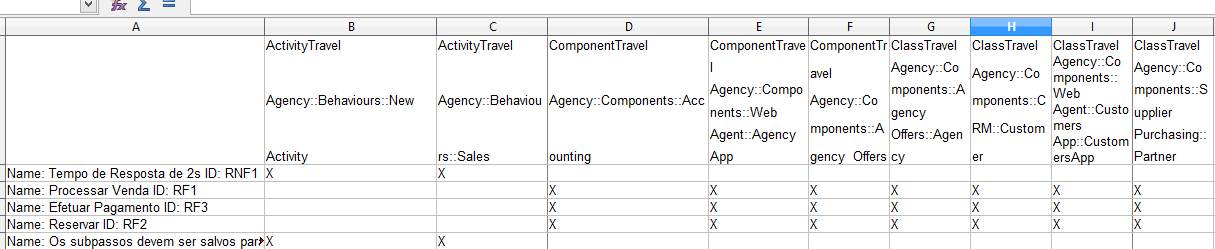
\includegraphics[width=.8\textwidth]{./images/matrixpart.png}
\caption{Parte da matriz de rastreabilidade gerada pela ferramenta}
\label{fig:matrixpart}
\end{figure}

Para gera��o de c�digo, utilizamos o \textit{plugin \gls{uml} to Java
Generator}, que por sua vez utiliza o ponto de extens�o do \textit{plugin
Acceleo}\footnote{http://www.eclipse.org/acceleo/}. O \textit{plugin
Acceleo} tem por finalidade transformar os modelos \gls{emf} em uma linguagem
definida pelo usu�rio, atrav�s de arquivos com a extens�o .mtl (\textit{Model
to Text Language}). Os arquivos .mtl possuem uma sintaxe pr�pria, que pode ser
vista no trecho de c�digo mostrado a seguir.

\begin{verbatim}
[comment encoding = UTF-8 /]
[module classifierJavaFile('http://www.eclipse.org/uml2/4.0.0/UML')]

[import org::obeonetwork::pim::uml2::gen::java::common::documentation /]
[import org::obeonetwork::pim::uml2::gen::java::common::path /]

[import org::obeonetwork::pim::uml2::gen::java::services::importService /]

[template private classifierJavaFilePath(aClassifier : Classifier)]
[if (not aClassifier.getNearestPackage().oclIsUndefined())]
[aClassifier.genPackagePath()/][aClassifier.name/].java
[else]
[aClassifier.name.concat('.java')/]
[/if]
[/template]
\end{verbatim}

Enquanto o \textit{Acceleo} tem por finalidade transformar modelos \gls{emf} em
uma linguagem pr�-definida pelo usu�rio, o plugin \textit{\gls{uml} to Java
Generator} tem a finalidade espec�fica de transformar modelos \gls{uml}
(persistidos como modelos \gls{emf}) em linguagem \textit{Java}. Ele n�o gera
apenas c�digo \textit{Java}, mas o projeto inteiro no \textit{Eclipse}, criando
as pastas, arquivos de configura��o, informa��es de importa��o e exporta��o,
ambiente de execu��o alvo, entre outros. Por este motivo tamb�m, o
\textit{plugin} \textit{\gls{uml} to Java
Generator} � bastante simples. As partes principais do \textit{plugin} s�o:

\begin{itemize}
  \item a \gls{ui},
especificando op��es de configura��o, como modelo \gls{uml} a ser utilizado, ambiente de execu��o
alvo, entre outras op��es;
  \item as classes de lan�amento do \textit{plugin Acceleo}, utilizando as
  informa��es da \gls{ui};
  \item os arquivos .mtl que descrevem como os modelos devem ser gerados, no
  caso, as informa��o de gera��os dos arquivos \textit{Java} e do projeto
  \textit{Eclipse}.
\end{itemize} 

As altera��es necess�rias para que o \textit{plugin \gls{uml} to Java Generator}
gerasse os coment�rios personalizados do modelo \textit{AccTrace} foram:

\begin{enumerate}
  \item altera��o da \gls{ui}, para que fosse poss�vel indicar o arquivo
  .acctrace;
  \item interven��o nas classes de lan�amento, para que o arquivo .acctrace
  fosse corretamente carregado e recuperado quando necess�rio;
  \item altera��o dos arquivos .mtl necess�rios para que o c�digo \textit{Java}
  gerado inclu�sse o(s) coment�rio(s) do modelo \textit{AccTrace}, se houver uma
  refer�ncia para o elemento \gls{uml} avaliado no momento.
\end{enumerate}

O coment�rio \textit{AccTrace} � recuperado usando \textit{query
invoke}\footnote{http://www.obeonetwork.com/page/the-acceleo-queries}, um
mecanismo utilizado pelo \textit{plugin Acceleo} que encapsula dentro dos
arquivos .mtl chamadas nativas a fun��es \textit{Java}. O \textit{query invoke}
usado foi inclu�do no arquivo
\textit{org.obeonetwork.pim.uml2.gen.java.services.typesServices.mtl} e �
descrito a seguir.

\begin{verbatim}
[query public getComment(anOclAny : OclAny) : String
	= invoke('org.obeonetwork.pim.uml2.gen.java.services.AccTraceServices', 
	'getComment(org.eclipse.emf.ecore.EObject)', Sequence{anOclAny}) /]
\end{verbatim}

No momento desejado (por exemplo, logo ap�s a constru��o da especifica��o de
uma classe ou interface) o \textit{query invoke} � chamado, passando como
argumento o objeto \gls{uml} avaliado no momento. Na classe \textit{Java
AccTraceServices} existe um m�todo \textit{getComment} que recebe como argumento
um objeto \textit{EObject}, ou seja, qualquer elemento \gls{emf}. Neste m�todo,
� verificado se o modelo \textit{AccTrace} foi especificado (em caso negativo,
nada � retornado). Logo em seguida, � verificado se no modelo \textit{AccTrace}
existe uma refer�ncia ao elemento \gls{uml} avaliado (significando que existe
uma associa��o entre um requisito, modelo e t�cnicas), e em caso positivo, o
coment�rio � constru�do e retornado, sendo inclu�do no corpo do c�digo
\textit{Java}. Caso o elemento \gls{uml} n�o seja encontrado no modelo, uma
\textit{String} vazia � retornada.

O coment�rio \textit{AccTrace} � constru�do utilizando a seguinte express�o
regular \textit{Java}:

\begin{verbatim}
String regex = "//!ACCTRACE!(/)?([^/\\\\0#]+(/)?)+#([^\\*\\*/])+";
\end{verbatim}

A op��o de se utilizar um coment�rio de linha (ao inv�s de coment�rios de
bloco, usados por exemplo pela documenta��o \textit{JavaDoc}) decorreu do fato
do coment�rio descrito ser inclu�do dentro do corpo da classe e m�todos, e caso
o programador decida comentar o trecho de c�digo inteiro, esse coment�rio n�o
atrapalharia essa opera��o.

Uma vez tendo os coment�rios personalizados nos c�digo-fonte Java, o \textit{plugin AccTrace} se encarrega de verificar os coment�rios
para traduz�-los em informa��es �teis ao desenvolvedor. O \textit{plugin} usa o ponto de extens�o \textit{Compilation Participant} da biblioteca \gls{jdt},
usado para acompanhar e recuperar informa��es �teis no processo de compila��o do c�digo. No caso deste trabalho, 
o ambiente entrega a \gls{ast} do modelo Java, e partir dele os coment�rios s�o extra�dos. Caso o coment�rio 
atenda � express�o regular de coment�rio do \textit{plugin AccTrace}, uma marca (\textit{marker}) � adicionada 
ao editor, indicando que naquele ponto h� um coment�rio v�lido. A marca replica o coment�rio, de modo que ao 
passsar o mouse sobre a marca, um \textit{popup} surge, conforme mostrado pela
Figura \ref{fig:acctracecomment}.

\begin{figure}[ht]
\centering
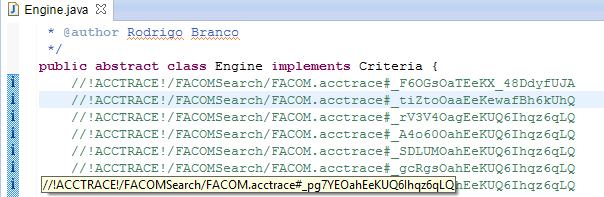
\includegraphics[width=.8\textwidth]{./images/acctracecomment.png}
\caption{Coment�rio padr�o AccTrace demonstrado utilizando o evento
\textit{mouse hover}}
\label{fig:acctracecomment}
\end{figure}

Ao clicar na marca, uma vis�o � notificada para que o conte�do do coment�rio
seja traduzido. A Figura \ref{fig:commentview} mostra um coment�rio j�
traduzido, onde se pode observar informa��es como requisito, modelo \gls{uml} e
quais t�cnicas est�o referenciadas por aquele coment�rio. A Figura
\ref{fig:commentrecovery} mostra como recuperar as informa��es relevantes
partindo de um coment�rio no formato AccTrace. O coment�rio passa por um
\textit{Regex Match}, sendo decomposto em:

\begin{itemize}
  \item Caminho relativo do arquivo do modelo AccTrace no \textit{workspace} do
  \textit{Eclipse};
  \item Refer�ncia (ID) da associa��o dentro do modelo;
\end{itemize}

O modelo AccTrace � carregado atrav�s do caminho encontrado e logo em seguida a
refer�ncia da associa��o � recuperada do modelo, usando seu ID como par�metro de
busca. A partir da ref�ncia � poss�vel recuperar o Requisito, o Modelo UML e as
t�cnicas de implementa��o de acessibilidade. Como no modelo AccTrace apenas as
refer�ncia aos objetos � armazenada, qualquer mudan�a nos objetos envolvidas �
vista em tempo real. A atualiza��o da tela da vis�o pode n�o ser
instant�nea, dependendo da complexidade dos objetos envolvidos e da quantidade
de recursos que devem ser recuperados.

\begin{figure}[ht]
\centering
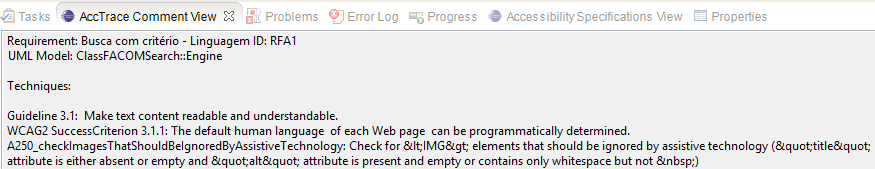
\includegraphics[width=.8\textwidth]{./images/commentview.png}
\caption{Vis�o de explicita��o do coment�rio selecionado.}
\label{fig:commentview}
\end{figure}

\begin{figure}[ht]
\centering
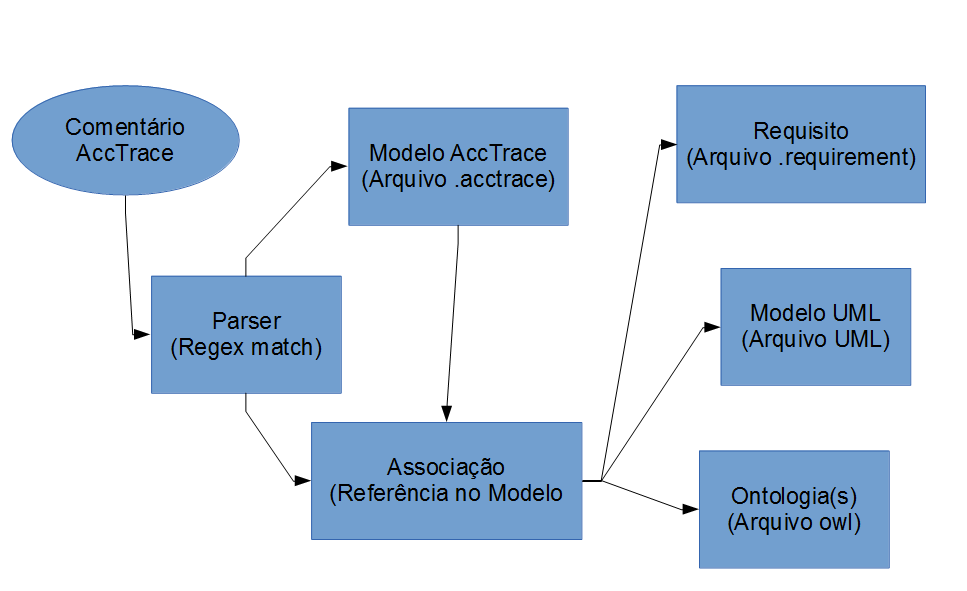
\includegraphics[width=.8\textwidth]{./images/commentrecovery.png}
\caption{Passos para recupera��o das informa��es relevantes atrav�s de um
coment�rio padr�o AccTrace}
\label{fig:commentrecovery}
\end{figure}


\chapter{Prova de Conceito}

Como prova de conceito, foi criado um projeto simples, de forma que utilize
o gls{mta}, bem como o \textit{plugin AccTrace}, assim
como os outros relacionados neste trabalho. Os atores aqui elencados s�o
fict�cios, tendo o especialista em acessibilidade os autores deste trabalho.
Objetivo aqui n�o � aplicar a prova de conceito no \gls{mta}, por isso nem todos
os artefados presentes no \gls{mta} ser�o constru�dos, e sim os artefatos utilizados por este trabalho.

\section{Defini��o do projeto}

O cliente solicitou a constru��o de um \textit{software} buscador. O objetivo
deste \textit{software} � fazer buscas na \textit{internet} utilizando como
chave uma ou mais palavras fornecidas pelo usu�rio.

O buscador ser� um software \textit{web}, sendo acessado atrav�s de navegadores.

\subsection{Subprocesso 1 - Elicita��o dos Requisitos do Sistema}

No subprocesso 1 (Elicita��o dos Requisitos do Sistema), observando a tarefa 1.1
do \gls{mta} (Identificar os Requisitos de Acessibilidade do Sistema), o
especialista em acessibilidade identificou que:

\begin{itemize}
  \item n�o existem caracter�sticas espec�ficas do usu�rio: todos usu�rios
  poder�o acessar o sistema, independente de habilidade e defici�ncias dos
  mesmos;
  \item como requisitos de dom�nio, foi identificado que o \textit{software}
  deve estar dispon�vel para a linguagem nativa do usu�rio, e caso ele prefira,
  a linguagem pode ser alterada. A busca deve ser influenciada pela escolha da
  linguagem;
  \item n�o existem requisitos tecnol�gicos espec�ficos: o sistema deve ser
  acessado indepentende de dispositivo ou tecnologia;
  \item requisito de performance: o sistema deve retornar o resultado em menos
  de 2 segundos, para n�o prejudicar a percep��o do usu�rio;
  \item requisito de conformidade: o sistema deve seguir a recomenda��o de
  acessibilidade \gls{wcag} 2.0, sem n�vel definido.
\end{itemize} 

Nenhum requisito funcional de acessibilidade foi identificado nesta etapa; at�
agora, o sistema deve seguir as boas pr�ticas gen�ricas de acessibilidade para
englobar todos os conjuntos de usu�rios/defici�ncias.

\subsection{Subprocesso 2 - An�lise de Requisitos do Sistema}

Partindo para o subprocesso 2 (An�lise de Requisitos do Sistema), na tarefa 2.1
(Especificar os Requisitos de Acessibilidade do Sistema), o especialista em
acessibilidade identificou que:

\begin{itemize}
  \item caracter�sticas do usu�rio: n�o existe um p�blico alvo definido. N�o �
  poss�vel inferir qual o n�vel de experi�ncia do p�blico alvo;
  \item requisitos de dom�nio: como ordem de execu��o de tarefas, o usu�rio deve
  informar a chave de pesquisa, recebendo o resultado no passo seguinte;
  \item requisitos de tecnologia: dependendo da defici�ncia/impedimento
  moment�neo do usu�rio, as tecnologias podem variar desde um leitor de tela at�
  o navegador textual. Isso deve ser considerado na utiliza��o do
  \textit{software};
  \item alternativas pr�-existentes: servi�os como Google, Bing ou Yahoo
  fornecem buscadores com os mesmo prop�sitos;
  \item qualidade das alternativas: o buscador do Google promove a busca
  acess�vel levando em considera��o alguns aspectos das p�ginas
  analisadas\footnote{https://support.google.com/websearch/answer/181196?hl=en},
  N�o foi identificado se o buscador Bing ou Yahoo possui algum mecanismo que
  avalie a acessibilidade das p�ginas avaliadas, apesar das duas empresas
  possu�rem �reas que tratam de quest�es de
  acessibilidade\footnote{http://yaccessibilityblog.com/ e
  http://www.microsoft.com/enable/}.
\end{itemize}

O especialista em acessibilidade constatou que 2 requisitos funcionais de
acessibilidade est�o presentes: o mecanismo de busca ser� alterado toda vez que
a linguagem padr�o for alterada, e o mecanismo de busca ser� alterado quando o
usu�rio informar suas necessidades espec�ficas, por exemplo, sua defici�ncia. As
duas abordagens podem ser desativadas caso o usu�rio preferir.

Nada mais pode ser dito sobre acessibilidade neste momento. Portanto, o
especialista me acessibilidade acrescentou como requisito n�o funcional: os
elementos do sistema devem ser: percept�veis, oper�veis, compreens�veis e robustos, seguindo os
princ�pios do \gls{wcag} 2.0. A avalia��o dos requisitos de acessibilidade �
feita na tarefa 2.2 (Avaliar os Requisitos de Acessibilidade do Sistema) e
registrada no documento de requisitos de acessibilidade do sistema
revisado.

\section{Modelagem do Sistema}

Os artefatos para que os desenvolvedores implementem o sistema come�am a surgir
a partir desta etapa.

\subsection{Subprocesso 3 - Projeto Arquitetural do Sistema}

No subprocesso 3 (Projeto Arquitetural do Sistema), as tarefas 3.1 (Alocar
Requisitos de Acessibilidade aos Elementos do Sistema) e 3.2 (Avaliar o Projeto Arquitetural do 
Sistema com Rela��o aos Requisitos de Acessibilidade) tratam da decomposi��o do
sistema em componentes menores, assim como a especifica��o da responsabilidade
de cada componente. Para os requisitos de acessibilidade descritos
anteriormente, � definido que, para cada um dos requisitos funcionais
(altera��o do mecanismo de busca), um componente individual ser� gerado, podendo
ter um elemento de renderiza��o gen�rico, ou um ou mais componentes de
renderiza��o para cada uma das altera��es do mecanismo de busca, ou at� da
combina��o delas.

O requisito n�o funcional identificado deve permear todos componentes do
projeto, inclusive os j� descritos anteriormente.

\subsection{Subprocesso 4 - An�lise de Requisitos do Software}

No subprocesso 4 (An�lise de Requisitos do Software), os requisitos de
acessibilidade do \textit{software} (interface e c�digo) s�o estabelecidos.

As taferas 4.1 (Estabelecer os Requisitos de Acessibilidade do Software) e
4.2 (Avaliar os Requisitos de Acessibilidade do Software) especificar, avaliar
e documentar os requisitos de sistema em requisitos de \textit{software}.
Todos os requisitos, tanto os funcionais (RF) como os n�o-funcionais (RNF), inclusive os d
e acessibilidade (RA), podem ser vistos abaixo:

\begin{itemize}
  \item o sistema deve permitir que, dado uma chave de busca (uma ou mais
  palavras), o resultado da busca seja retornado (RF);
  \item o sistema deve permitir que o usu�rio altere a linguagem padr�o da
  ferramenta (RF);
  \item o sistema deve permitir que o usu�rio altere o constraste da p�gina
  (RF);
  \item o sistema deve permitir que o usu�rio altere o tamanho da fonte da
  p�gina (RF);
  \item o sistema deve utilizar a linguagem especificada como crit�rio de
  sele��o no mecanismo de busca (RF e RA);
  \item o sistema deve permitir que o usu�rio informe qual � o tipo de
  limita��o/defici�ncia possui (RF);
  \item o sistema deve utilizar o tipo de limita��o/defici�ncia como crit�rio de
  sele��o no mecanismo de busca (RF e RA);
  \item o sistema deve retornar o resultado da busca em menos de 2 segundos,
  para n�o prejudicar a percep��o do usu�rio (RNF);
  \item o sistema o sistema deve seguir a recomenda��o de
  acessibilidade \gls{wcag} 2.0, n�vel AAA (RNF e RA);
  \item o sistema deve fornecer componentes percept�veis, oper�veis,
  compreens�veis e robustos (RNF e RA);
  \item o sistema deve fornecer atalhos via teclado, para alterar o idioma e a
  informa��o sobre a limita��o/defici�ncia, sempre voltando o foco para a caixa
  de texto principal (RF);
  \item o sistema deve permitir que todas as funcionalidades sejam acess�veis
  via teclado (RF e RA);
  \item o sistema deve permitir que o tempo para ler utilizar o conte�do seja
  suficiente (RNF e RA);
  \item o sistema deve entregar um conte�do que n�o cause apreens�o (RNF e RA);
  \item o sistema deve permitir que o usu�rio navegue facilmente e
  encontre o conte�do desejado (RNF e RA);
  \item o sistema deve permitir que, ao ser especificado o tipo de
  limita��o/defici�ncia, a utiliza��o de m�tricas de acessibilidade sejam
  utilizadas para classificar as p�ginas (RF e RA).
\end{itemize}

No \textit{plugin Requirement Designer}, os requisitos s�o agrupados em 2
categorias principais: Requisitos Funcionais e Requisitos N�o Funcionais. Cada
uma dessas categorias possui uma categoria de agrupamento dos requisitos de
acessibilidade. A Figura \ref{fig:facomsearchrequirementplugin} mostra o
cadastro dos requisitos na ferramenta.

\begin{figure}[ht]
\centering
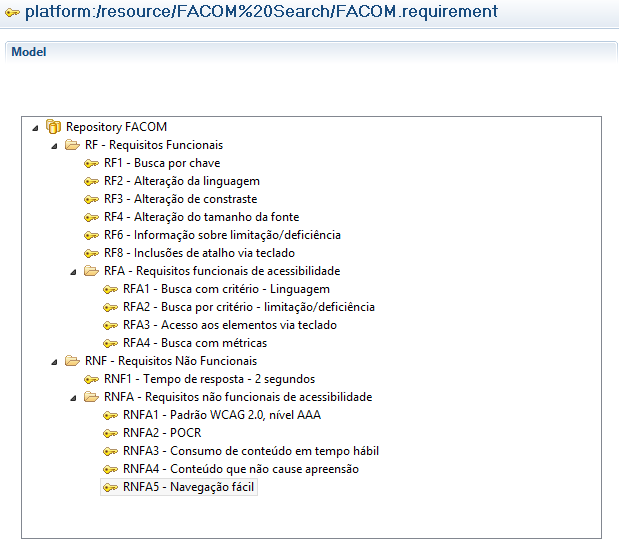
\includegraphics[width=.8\textwidth]{./images/facomsearchrequirementplugin.png}
\caption{Cadastro dos requisitos no \textit{plugin Requirement Designer}}
\label{fig:facomsearchrequirementplugin}
\end{figure}

O diagrama de casos de uso pode ser visto na Figura
\ref{fig:facomsearchusescase}, assim como o diagrama de classes pode ser visto
na Figura \ref{fig:facomsearchclassdiagram}. Como a implementa��o final deste
projeto n�o � o foco deste trabalho, as especifica��es dos casos de uso, assim
como outros diagramas \gls{uml} que n�o s�o transformados
no c�digo final n�o ser�o constru�dos. O diagrama de casos de uso aqui
apresentado tamb�m n�o � usado pelo gerador de c�digo, mas pela import�ncia do
artefato entendeu-se que era necess�rio a constru��o do mesmo.

\begin{figure}[ht]
\centering
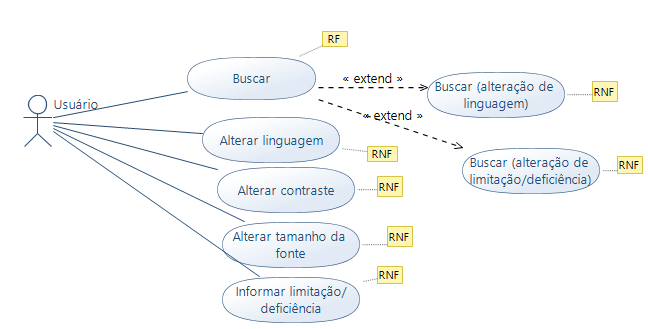
\includegraphics[width=.8\textwidth]{./images/facomsearchusescase.png}
\caption{Diagrama de casos de uso do buscador}
\label{fig:facomsearchusescase}
\end{figure}

\begin{figure}[ht]
\centering
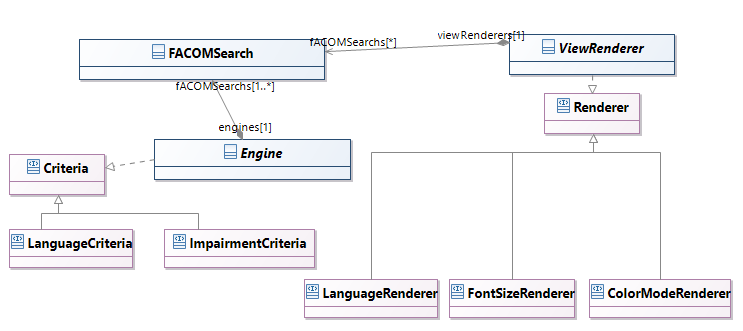
\includegraphics[width=.8\textwidth]{./images/facomsearchclassdiagram.png}
\caption{Diagrama de classes do buscador}
\label{fig:facomsearchclassdiagram}
\end{figure}

Vale notar que o \gls{mta} n�o especifica exatamente quando os diagramas
apresentados devem ser constru�dos. Por este motivo, o momento oportuno para a
constru��o dos mesmos foi entre os subprocessos 4 e 5, pela gama de informa��es
j� levantada.

De posse dos diagramas \gls{uml}, j� � poss�vel associ�-los aos requisitos,
utilizando o \textit{plugin Requirement Designer}. Com os requisitos e modelos
\gls{uml} j� associados, o arquivo .acctrace pode ser criado, recebendo como
entrada o arquivo .requirement. A Figura \ref{fig:referenciascriadas} mostra os
modelos \gls{uml}, para o modelo selecionado, os requisitos que a ele est�o
associados.

\begin{figure}[ht]
\centering
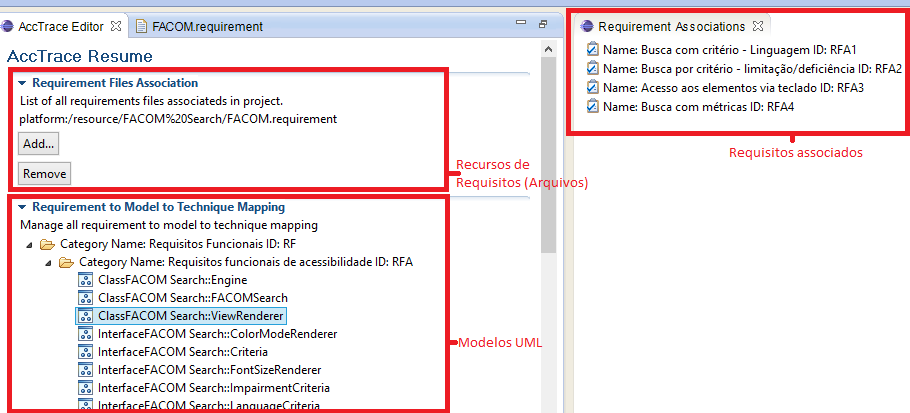
\includegraphics[width=.8\textwidth]{./images/referenciascriadas.png}
\caption{Modelos \gls{uml} e requisitos associados}
\label{fig:referenciascriadas}
\end{figure}

\subsection{Subprocesso 5 - Projeto de Software}

O subprocesso 5 (Projeto de \textit{Software}) visa fornecer um projeto onde os requisitos do software possam ser
implementados e verificados. Os elementos de interface s�o definidos nas
tarefas seguintes (Tarefa 5.1 - Projetar Interfaces Externas Acess�veis e
Tarefa 5.2 - Realizar Projeto Navegacional Acess�vel), e \citet{maia:10}
consegue estabelecer relacionamentos com o \gls{wcag} 2.0 nestas tarefas. Por
este motivo, mostrou-se adequado especificar as t�cnicas de acessibilidade neste
momento. Na subtarefa 5.2.1 (Estabelecer a disposi��o dos elementos na
interface), por exemplo, � citado 3 crit�rios de sucesso

\begin{itemize}
  \item \textbf{crit�rio de Sucesso 1.3.1 - Informa��es e Relacionamento:} A informa��o,
estrutura e relacionamento transmitido por meio de apresenta��o devem ser
determinados programaticamente;
  \item \textbf{crit�rio de Sucesso 1.3.2 - Sequ�ncia Significativa:} A sequ�ncia correta de
leitura dos elementos da interface deve ser determinada programaticamente;
  \item \textbf{crit�rio de Sucesso 1.3.3 - Caracter�sticas Sensoriais:} As instru��es
fornecidas para o entendimento e opera��o do conte�do n�o devem confiar
somente em caracter�sticas sensoriais dos componentes, tais como forma,
tamanho, localiza��o visual, orienta��o ou som.
\end{itemize}

enquanto a subtarefa 5.2.2 (Definir as cores dos elementos), sugere
um crit�rio de sucesso

\begin{itemize}
  \item \textbf{crit�rio de Sucesso 1.4.1 - Uso de Cores:} As cores n�o devem ser usadas
como �nico meio para transmitir informa��o, indicar uma a��o, mostrar uma
resposta ou distinguir um elemento visual.
\end{itemize}

e a subtarefa 5.2.1 (Definir a ordem de navega��o dos objetos) sugere um
crit�rio de sucesso

\begin{itemize}
  \item \textbf{crit�rio de Sucesso 2.4.3 - Ordem do Foco:} Se a p�gina Web pode ser
navegada sequenciamente e a sequ�ncia de navega��o afeta o entendimento ou
opera��o, ent�o os componentes focaliz�veis devem receber o foco considerando
a ordem dos elementos, preservando o entendimento e a operabilidade dos
mesmos.
\end{itemize}

\citet{maia:10} n�o especificou nenhum crit�rio de sucesso para a subtarefa
subtarefa 5.2.2 (Definir atalhos de navega��o), mas � poss�vel sugerir
genericamente um que sirva como ponto de partida:

\begin{itemize}
  \item \textbf{crit�rio de Sucesso 2.1.1 - Teclado:} Toda a funcionalidade do conte�do � oper�vel 
  atrav�s de uma interface de teclado sem requerer temporiza��es espec�ficas para digita��o individual, 
  exceto quando a fun��o subsequentes requer entrada que depende do caminho do
  movimento do usu�rio e n�o apenas dos pontos finais.
\end{itemize}

Os crit�rios de sucesso aqui apresentados s�o sugest�es e podem ou n�o ser
utilizados dependendo da situa��o. Neste ponto, podemos especificar as t�cnicas
de acessibilidade no \textit{plugin AccTrace}. � importante notar que n�o apenas
crit�rios de sucesso que est�o presentes no \textit{plugin}; todas as
abordagens, diretrizes, t�cnicas, entre outros (definidos nos arquivos de
ontologia) est�o dispon�veis para a associa��o, dependendo apenas das
caracter�sticas espec�ficas do projeto e da maturidade do especialista em
acessibilidade.



\chapter{Conclus�es}

\section{Considera��es Iniciais}

Este cap�tulo apresenta as conclus�es gerais desta disserta��o, bem como as
contribui��es e trabalhos futuros.

\section{Contribui��es do Trabalho}

O tema \textit{Acessibilidade no Processo de desenvolvimento de software} ainda
� pouco explorado, com poucos trabalhos publicados a respeito
\citep{maia:10,5599835}. Em contrapartida, podemos encontrar diversos
estudos que dizem respeito ao rastreamento de requisitos
\citep{5970169,292398,5485417,6405269}, bem como encontrar estudos que utilizam
ontologias para o mapeamento do dom�nio no processo de desenvolvimento ou na
rastreabilidade dos requisitos \citep{5223183,6511842,4148940,5362244}. Contudo,
n�o foi encontrado na literatura estudos espec�ficos sobre a rastreabilidade de
requisitos de acessibilidade durante o processo de desenvolvimento de \textit{software}.

Al�m disso, este estudo mostrou ser poss�vel
especificar, antes das fases de codifica��o e vinculadas aos modelos e
requisitos de acessibilidade, as t�cnicas de implementa��o que dever�o
ser visualizadas pelos programadores. A utiliza��o de ontologias pr�-definidas
do projeto \citet{aegis:13} ajudou a alcan�ar tal objetivo, estendendo as
t�cnicas de implementa��o anteriormente ditas para abordagens, diretrizes,
crit�rios de sucesso, entre outros.

Este estudo n�o tem por objetivo entregar uma ferramenta \gls{case} que atenda
�s exig�ncias aqui descritas; o objetivo principal � discutir as maneiras em que
a rastreabiliade pode ser promovida (utilizando t�cnicas j� descritas na
literatura e utilizadas em outros trabalhos), e a partir das v�rias op��es
dispon�veis, escolher a mais adequada, levando em considera��es a ferramentas
dispon�veis, contexto abordado e limita��es inerentes.

Como j� dito por \citet{maia:10}, este trabalho pressup�e que um especialista
em acessibilidade participe do processo de desenvolvimento, principalmente nas
subtarefas de acessibilidades proposta pelo \gls{mta}. A proposta deste trabalho
pode se estender para outras �reas (por exemplo, usabilidade, seguran�a, etc),
desde que haja um especialista e que o dom�nio esteja mapeado na forma de
ontologias, ou outro formato que possa ser interpretado por uma ferramenta
\gls{case}. Obviamente, a ferramenta aqui apresentada, da maneira como est�, n�o
poderia ser usada para tal prop�sito, mas pode ser modificada para que se adeque
� essa situa��o, pois � poss�vel perceber que a grande complexidade n�o � a
ferramenta em si, mas sim possuir o especialista e o dom�nio mapeado.

� poss�vel apontar, portanto, tr�s grandes contribui��es fornecidas por este
trabalho:

\begin{enumerate}
  \item abordar o rastreamento dos requisitos de acessibilidade em um processo
  de desenvolvimento que inclui tarefas de acessibilidade (\gls{mta});
  \item permitir a especifica��o de t�cnicas de implementa��o de acessibilidade, 
  mapeadas em ontologias pr�-definidas;
  \item fornecer uma ferramenta como prova de conceito que possa ser
  alterada/aprimorada para trabalhos futuros.
\end{enumerate}

\section{Participa��es em eventos}

Este trabalho teve sua import�ncia reconhecida atrav�s da sele��o para
participa��o, como trabalho de p�s-gradua��o em andamento, e apresenta��o de
poster no \textit{PASQI Workshop}, realizado em Costa Rica e patrocinado por:
\textit{Michigan Technological University, Pontificia Universidad Cat�lica de
Chile, Miami University, Universidad de Buenos Aires, Universidad de Chile e
Universidad de Costa Rica}.

\section{Trabalhos Futuros}

� poss�vel identificar v�rias abordagens para trabalhos futuros:

\begin{itemize}
  \item efetuar um estudo de caso com um projeto real, que utilize o \gls{mta} e
  use os \textit{plugins} aqui elencados, inclusive os \textit{plugins}
  constru�dos e customizados para promover a rastreabilidade e gera��o de
  c�digo;
  \item efetuar um estudo de caso com usu�rios reais, utilizando o
  \textit{software} constru�do no item anterior e avaliar a acessibilidade do
  mesmo;
  \item estudar a utiliza��o de m�todos din�micos de rastreabilidades dos
  requisitos;
  \item efetuar o mapeamento das ontologias para outros documentos de refer�ncia
  em acessibilidade, por exemplo, eMag 3.0;
  \item aumentar a usabilidade dos \textit{plugins} constru�dos/modificados,
  melhorando as mensagens apresentadas, aproveitando o relacionamento das
  ontologias do projeto \citet{aegis:13};
  \item estender o escopo deste trabalho, inclu�ndo tarefas de testes e
  integra��o do \textit{software} e do sistema (subtarefas 7, 8, 9 e 10 do
  \gls{mta});
  \item estender a matriz de rastreabilidade dos requisitos aqui constru�da,
  para incluir os casos de testes descritos no item anterior;
  \item utilizar outro dom�nio de interesse como base para os estudos futuros,
  como por exemplo usabilidade de \textit{software}.
\end{itemize}
%\chapter{Proposta de trabalho}

O levantamento bibliogr�fico mostrou que a �rea de acessibilidade em
sistemas \textit{web} ainda apresenta grandes desafios. Entre eles, podemos
citar:

\begin{itemize}
  \item entregar produtos acess�veis que cubram 100\% das
  defici�ncias e dificuldades;
  \item testar a acessibilidade dos \textit{sites};
  \item implementar plenamente as diretrizes de acessibilidade nos produtos;
  \item mensurar o qu�o acess�vel um \textit{site} �;
  \item escolher a melhor m�trica de avalia��o de acessibilidade;
  \item definir arquiteturas de produtos e servi�os j� existentes de forma que
  agreguem acessibilidade;
  \item conscientizar o desenvolvedor da import�ncia da acessibilidade nos
  produtos;
  \item fornecer ambientes que de fato auxiliem desenvolvedores a entregar
  produtos acess�veis.
\end{itemize}

Podemos observar que os desafios citados anteriormente se relacionam com o
usu�rio final ou com o desenvolvedor. Neste trabalho, optou-se por escolher
a abordagem do desenvolvedor, confeccionando uma ferramenta (\textit{plugin})
para o ambiente de desenvolvimento integrado \textit{Eclipse}.

O trabalho foi motivado pela pesquisa realizada por
\cite{Trewin:2010:ACT:1805986.1806029}, indicando a insatisfa��o dos
desenvolvedores com as ferramentas dispon�veis de desenvolvimento, considerando
a integra��o de acessibilidade ao produto.
Os autores j� possuem experi�ncia com uma ferramenta de avalia��o de \textit{sites} \citep{branco:09}, bem como a
utiliza��o de m�tricas de acessibilidades na avalia��o \citep{branco:11}. Essa
experi�ncia ser� �til para o desenvolvimento do trabalho.

\section{Cronograma}

As atividades abaixo relacionadas ser�o executadas como parte da
metodologia para que os objetivos sejam alcan�ados:

\begin{enumerate}
  \item complementar a pesquisa bibliogr�fica;
  \item escrever e apresentar a qualifica��o;
  \item identificar os pontos de integra��o entre as atividades de Engenharia de
  Requisitos e gera��o de c�digo;
  \item estudar a confec��o de \textit{plugins} para o \textit{Eclipse};
  \item criar e integrar o \textit{plugin} com o \textit{Eclipse};
  \item efetuar testes preliminares da ferramenta;
  \item comparar com outras ferramentas existentes;
  \item efetuar estudos de caso utilizando a ferramenta desenvolvida;
  \item analisar os resultados;
  \item elaborar e publicar artigos cient�ficos;
  \item escrever e defender a disserta��o.
\end{enumerate}

O cronograma das atividades que j� foram
realizadas neste trabalho e as atividades previstas � apresentado a seguir,
considerando as tarefas elencadas anteriormente.

\begin{figure}[ht]
\centering
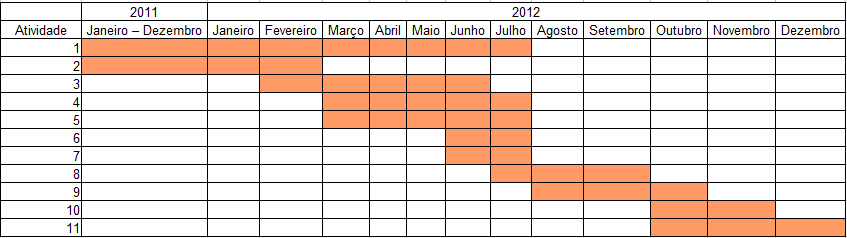
\includegraphics[width=1.0\textwidth]{./images/cronograma.png}
\caption{Cronograma das atividades}
\label{fig:cronograma}
\end{figure}
%---------------------------------------------------------------------
% Aqui est� um exemplo de bibliografia
% Veja o arquivo bibi_exemplo.bib
% Para voc� ter um " GUIA "
%---------------------------------------------------------------------
\refstepcounter{chapter}
\refstepcounter{chapter}% Adiciona 1 to chapter ou seja (\thechapter=\thechapter+1)

\addcontentsline{toc}{chapter}{Bibliografia}\label{bibliografia}
%\nocite{*}

%-----
% Define o estilo das refer�ncias bibliogr�ficas
%-----
\bibliographystyle{apalike}
%
%\nocite{*}

\bibliography{sbc-template}
%--------------------------------------------------------------------
\end{document}
